\documentclass[lettersize,journal]{IEEEtran}
\usepackage{amsmath,amsfonts}
\usepackage{algorithmic}
\usepackage{algorithm}
\usepackage{array}
\usepackage[caption=false,font=normalsize,labelfont=sf,textfont=sf]{subfig}
\usepackage{subcaption}
\usepackage{textcomp}
\usepackage{stfloats}
\usepackage{url}
\usepackage{verbatim}
\usepackage{graphicx}
\usepackage{tikz}
\usetikzlibrary{automata, positioning}
\usepackage{cite}
\hyphenation{op-tical net-works semi-conduc-tor IEEE-Xplore}
% updated with editorial comments 12/2/2022

\begin{document}

\title{Journal DAO: \\ User-Incentivized Autonomous Decentralized Scientific Publishing in Web3}

\author{Tai Jiang, Rui Qin,~\IEEEmembership{Member, IEEE}, Yuhang Liu, \\
  Fei-YueWang,~\IEEEmembership{Fellow,~IEEE}.
  % <-this % stops a space
  \thanks{This work was supported by the Science and Technology Development Fund of Macau SAR under Grant 0093/2023/RIA2 and  Grant 0050/2020/A1.}% <-this % stops a space
  \thanks{Manuscript received February 15, 2023; revised February 15, 2023.}
  \thanks{Tai Jiang is with the Department of Engineering Science, Faculty of Innovation Engineering, Macau University of Science and Technology, Macao, 999078, China (e-mail: jiangtai20@mails.ucas.ac.cn).}
  \thanks{Rui Qin is with Institute of Automation, Chinese Academy of Sciences, Beijing 100190, China (e-mail: rui.qin@ia.ac.cn).}
  \thanks{Yuhang Liu is with the State Key Laboratory for Management and Control of Complex Systems, Institute of Automation, Chinese Academy of Sciences, Beijing 100190, China, and also with the School of Artificial Intelligence, University of Chinese Academy of Sciences, Beijing 100049, China (e-mail: liuyuhang21@mails.ucas.ac.cn).}
  \thanks{Fei-Yue Wang is with the State Key Laboratory for Management and Control of Complex Systems, Chinese Academy of Sciences, Beijing 100190, China, and also with the Macao Institute of Systems Engineering, Macau University of Science and Technology, Macao 999078, China (e-mail: feiyue.wang@ia.ac.cn).}

}

% The paper headers
\markboth{Journal of \LaTeX\ Class Files,~Vol.~14, No.~8, February~2023}%
{Shell \MakeLowercase{\textit{et al.}}: A Sample Article Using IEEEtran.cls for IEEE Journals}

% \IEEEpubid{0000--0000/00\$00.00~\copyright~2021 IEEE}
% Remember, if you use this you must call \IEEEpubidadjcol in the second
% column for its text to clear the IEEEpubid mark.

\maketitle

\begin{abstract}

  The academic publishing industry is currently undergoing significant growth but also faces several challenges, mainly including the lack of transparency in the peer review process and the limited rights of authors. The rise of Web3, emphasizing decentralization, openness, and user control over data, opens up new perspectives for academic publishing. This article introduces an innovative academic publishing model, named Journal DAO, leveraging emerging Web3 technologies such as blockchain and decentralized autonomous organization (DAO). First, by recording articles on the blockchain rather than a centralized database, Journal DAO can ensure data security and traceability of the articles. Second, through the governance framework of DAO, tokens are distributed among all the participants of Journal DAO based on the their contributions, safeguarding the rights of each role in the publishing process. Third, effective incentive mechanisms are proposed to reward all participants, ensuring the sustainability of the framework and its autonomous functionality. This work proposes a prospective academic publishing model that aims to reshape the industry through the application of blockchain and DAO in Web3, making a significant contribution to future academic publishing.


\end{abstract}


\begin{IEEEkeywords}
  Decentralized autonomous organizations, blockchain, Web3.0, decentralized funding, decentralized science
\end{IEEEkeywords}

\section{Introduction \label{sec:introduction}}


\IEEEPARstart{T}{he} academic publishing industry is currently facing several pressing challenges. First, the traditional system, often conducted anonymously, fails to ensure fairness and impartiality, leading to a compromised review process that undermines both credibility and integrity. This lack of transparency can undermine the credibility and integrity of the review process. Second,
the authors often lack control over associated data of their articles, since the ownership often rests with publishers or electronic databases \cite{lancaster1995evolution}. This challenges authors in retaining rights, deciding on data use, and hampers their ability to fully leverage research, limiting collaborative opportunities and further advancements in their field. Third, the restrictions on data sharing hinder the free flow of knowledge and inhibit potential collaborations, which limits authors from fully benefiting and making discoveries that could contribute to the scientific community.
% 学术出版行业目前面临着几个紧迫的挑战。首先，传统的系统通常是匿名进行的，无法确保公平和公正，导致审查过程受到损害，从而损害了可信度和完整性。这种缺乏透明度可能会损害审查过程的可信度和完整性。其次，作者通常无法控制其文章的相关数据，因为所有权通常属于出版商或电子数据库。这对作者保留权利、决定数据使用提出了挑战，并妨碍了他们充分利用研究成果的能力，限制了合作机会和其领域的进一步发展。第三，对数据共享的限制阻碍了知识的自由流动并抑制了潜在的合作，这限制了作者充分受益并做出可能对科学界做出贡献的发现。

The emergence of technologies such as Decentralized Autonomous Organizations (DAOs) \cite{buterin2014next} and blockchain \cite{swan2015blockchain,9093840} presents significant opportunities for the advancement of the academic publishing industry. DAOs offer a groundbreaking approach to organizational governance, decision-making, and fund management for academic publishing \cite{wang2019decentralized}. Unlike traditional hierarchical structures, DAOs operate without central authorities, relying on transparent and automated processes governed by smart contracts and consensus protocols \cite{kaal2021decentralized}. This decentralization can provide a transparent and auditable decision-making process, enhance accountability, and facilitate efficient funds distribution for the current academic publishing system. The decentralized and tamper-resistant nature of blockchain can provide a secure and transparent environment for intelligent journals. By integrating blockchain technology into intelligent journals, the data transparency and authenticity can be realized. Through blockchain-based smart contracts, the reliability of data can be steadfastly guaranteed, thereby eliminating the necessity for third-party oversight \cite{mougayar2016business}. This innovative approach not only enhances the credibility of information but also streamlines the process, fostering trust and efficiency within the realm of intelligent journals.
% 去中心化自治组织(DAO)等技术的出现为学术出版行业的发展提供了重大机遇。DAO 为学术出版的组织治理、决策和资金管理提供了一种开创性的方法。与传统的层级结构不同，DAO 的运作没有中央权威，而是依靠由智能合约和共识协议管理的透明和自动化流程。这种去中心化可以提供透明和可审计的决策过程，加强问责制，并促进当前学术出版系统的有效资金分配。区块链的去中心化和防篡改特性可以为智能期刊提供安全透明的环境。通过将区块链技术集成到智能期刊中，可以实现数据的透明度和真实性。通过基于区块链的智能合约，数据的可靠性可以得到坚定的保证，从而消除第三方监督的必要性。这种创新方法不仅提高了信息的可信度，还简化了流程，在智能期刊领域促进了信任和效率。

In the literature, the applications of blockchain-based decentralized technologies in academic publishing have received researchers' great attention \cite{8756390}. Blockchain technology was used to solve the security and efficiency concerns in the distribution and management of open journal systems, ensuring precise distribution, enhancing reputation and trust, and safeguarding paper management against potential hacker threats \cite{agustin2020blockchain}. Through decentralized InterPlanetary File System (IPFS) and blockchain technologies, the authenticity, trust and reliability of online publications can be ensured, which can effectively address the challenges related to security and privacy in online publications \cite{nizamuddin2018ipfs}. By leveraging blockchain-based decentralized technologies, a decentralized scientific publishing platform is established, which utilizes Ethereum smart contracts to expedite the publication process, reduce biases in peer review, and lower publication costs \cite{becstacs2023novel}. The platform can ensure complete traceability throughout the publication processes, and all the participants including the editors, reviewers, and authors will receive system tokens as rewards for their contributions.
% 在文献中，基于区块链的去中心化技术在学术出版中的应用受到了研究人员的高度关注。区块链技术用于解决开放期刊系统分发和管理中的安全性和效率问题，确保精确分发，增强声誉和信任，并保护论文管理免受潜在的黑客威胁。通过去中心化的星际文件系统 (IPFS) 和区块链技术，可以确保在线出版物的真实性、信任度和可靠性，从而有效解决在线出版物中与安全和隐私相关的挑战。通过利用基于区块链的去中心化技术，建立了一个去中心化的科学出版平台，该平台利用以太坊智能合约来加快出版流程，减少同行评审中的偏见，并降低出版成本。该平台可以确保整个出版过程的完整可追溯性，所有参与者，包括编辑、审稿人和作者都将获得系统代币作为其贡献的奖励。

However, these existing studies primarily concentrate on specific aspects, such as the use of blockchain to address security and efficiency concerns or enhance transparency in the academic publishing process. They do not comprehensively address the multifaceted challenges prevalent in the current academic publishing landscape. This article proposes an innovative academic publishing model called Journal DAO, which applies emerging Web3 technologies, such as blockchain and DAO, to address these challenges. First, by recording articles on the blockchain, all operations are conducted on the chain rather than belonging to a specific database, ensuring data security and traceability. Second, through the DAO framework, tokens are distributed based on role contributions, protecting the rights of researchers. Third, by designing effective incentive mechanisms, with the consideration of rewarding each participant according to their contributions to the article, a fully autonomous and economically sustainable Journal DAO ecosystem can be realized \cite{ding2022desci}.
% 但现有研究主要集中于某些方面，如利用区块链解决安全性和效率问题或增强学术出版流程的透明度，并未全面解决当前学术出版领域普遍存在的多方面挑战。本文提出了一种创新的学术出版模式——Journal DAO，利用区块链、DAO 等新兴的 Web3 技术来解决这些挑战。首先，通过将文章记录在区块链上，所有操作都在链上进行，而不属于某个特定的数据库，确保数据的安全性和可追溯性。其次，通过 DAO 框架，根据角色贡献度进行 Token 分配，保护研究人员的权益。第三，通过设计有效的激励机制，考虑根据每个参与者对文章的贡献进行奖励，实现完全自治且经济可持续的 Journal DAO 生态系统。

The rest of this paper is arranged as follows. Section \ref{sec:framework} introduces the framework of Journal DAO framework. Section \ref{sec:mechanism} discusses the design and implementation of the incentive mechanism in Journal DAO. Section \ref{sec:performance} presents experimental results validating the effectiveness of the implemented incentive mechanism.
Section \ref{sec:conclusion} concludes the paper.
% 本文的其余部分安排如下。\ref{sec:framework} 节介绍了 Journal DAO 框架的框架。\ref{sec:mechanism} 节讨论了 Journal DAO 中激励机制的设计和实现。\ref{sec:performance} 节介绍了验证所实施激励机制有效性的实验结果。\ref{sec:conclusion} 节对本文进行了总结。

% 第2节之前的内容共1.25页

\section{Framework of Journal DAO \label{sec:framework}}

% 第2节共2.25页
% 开头写一段话，介绍本节主要做什么，2-3行即可。




% \subsection{The Framework}1页

% 本小节给出Journal DAO的framework，建议画一张框架图，图中要包含所有参与者，还要包含完整的运行流程，以及token和finance的流转。

% 在框架图的基础上，简要介绍框架图，并说明区块链和DAO在其中如何发挥作用。

% \subsection{The Operation Process}1页

% 介绍Journal DAO框架中参与者的各类角色，Journal DAO运行流程和实现的功能，以及token和finance如何流转。

% \subsection{The Advantages}0.25页

% 介绍与传统期刊相比，Journal DAO有哪些优势.

% \section{Mechanism Design of Journal DAO \label{sec:mechanism}}本节共2页
% 简要写一下本节的思路，3-5行即可。

% \subsection{Decentralized Governance}

% \subsection{Initial Token Distributions}

% \subsection{Token Distributions upon Article Download or Citation}

% \subsection{Finance Distributions}

% \section{A Case Study} \label{sec:performance}本节共2页

% \section{Conclusions and Future Work\label{sec:conclusion}}共0.25页

% 第一段，对本文的工作进行总结。

% 第二段，对下一步的工作进行展望。

% \bibliography{refs}1页
% \bibliographystyle{IEEEtran}

% 作者简介：0.75页


%  

This chapter present the implementation details and methodology of the web3-based Journal DAO system, which combines blockchain technology, smart contracts, and decentralized science(DeSci) practices. The system's design and development are rooted in the utilization of Non-Fungible Tokens (NFTs) and Recursive Inscriptions to establish a robust incentive framework that benefits all participants. This chapter delves into the technical aspects of the system, outlining the steps taken to create a self-governing and autonomous journal ecosystem. Additionally, the methodology employed for the integration of blockchain, smart contracts, and decentralized scientific practices is discussed in detail. Through a comprehensive exploration of the implementation and methodology, this chapter offers insights into the practical application of the proposed Journal DAO system and its potential to transform traditional journal publication models.
% 本文在区块链的基础上，利用智能合约，结合去中心化科学，创建一个基于web3的journal DAO系统。系统基于NFT以及递归铭文制定了一套激励机制，让所有参与者都获利，最终杂志系统自治。



\subsection{The Framework}
% \subsection{The Framework}1页
% 本小节给出Journal DAO的framework，建议画一张框架图，图中要包含所有参与者，还要包含完整的运行流程，以及token和finance的流转。
% 在框架图的基础上，简要介绍框架图，并说明区块链和DAO在其中如何发挥作用。
% A节，简要介绍该框架，比如有哪些核心参与者，有哪些关键环节等，不需要详细介绍这些环节，详细的介绍可以放在B节中。



Based on the depicted framework in Figure \ref{fig:frameworkofblockchain}, it is evident that the operational flow of the blockchain and DAO framework, along with the roles of various participants \cite{10459713}, can be succinctly understood.
%基于图中描绘的框架，显然可以简洁地理解区块链和 DAO 框架的操作流程，以及各个参与者的角色。


\begin{figure}[h!]
  \centering
  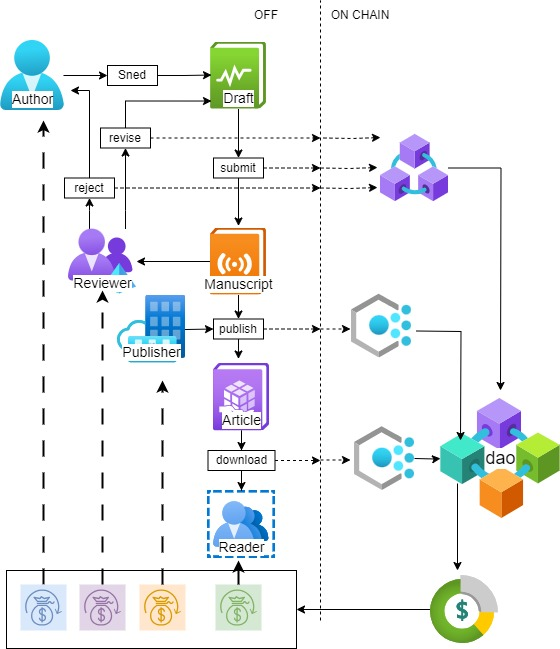
\includegraphics[width=\linewidth]{assets/frame.jpg}
  \caption{Framework of Blockchain.}
  \label{fig:frameworkofblockchain}
\end{figure}

In the DeSci framework, the core participants closely resemble those in traditional web2.0 journals. These include article authors, categorized as first author, second author, and so forth, as well as corresponding authors. The framework also involves peer reviewers, such as Editors in Chief (EIC), Senior Editors (SE), Associate Editors (AE), and more normal Reviewers. Readers form another essential group, who can download articles and even become authors themselves by citing and downloading referenced papers. Additionally, there are publishers representing the journal.
The submission process, review assignment, rejection, and final publication in this DeSci framework exhibit minimal differences from traditional journals. Similarly, readers can download articles without significant distinctions from web2.0 journals. However, within this framework, the requirement for cited articles to be downloaded ensures the smooth operation of the DAO Framework, guaranteeing the integrity and functionality of the decentralized ecosystem.
% 在去中心化科学框架中，核心参与者跟传统web2.0杂志没有太多区别，有文章的作者，一作、二作……通讯作者；有审稿人，Editors in Chief(EIC)、Senior Editor(SE)、Associate Editor(AE)，以及多个普通审稿人；有读者，读者可能下载论文，也可能成为一个新的作者引用下载的论文；还有代表杂志的出版商。作者投稿，EIC分配审稿人，退稿，以及最终发布，从流程上几乎没有区别。读者下载论文，也跟web2。0杂志一样，然而，本框架用区块链技术强调了知识的价值。


In the DAO framework \cite{hsieh2018bitcoin}, token allocation follows a process where all participants, including authors, reviewers, readers, and publishers, are assigned contributions represented by tokens. This allocation is carried out based on the established procedures within the framework.
Within this context, NFTs can be utilized as a means to determine the distribution proportions of tokens. NFTs are unique tokens that represent specific assets or contributions \cite{10034436}. By employing NFTs, the token allocation process becomes more granular, allowing for a more precise distribution based on the individual contributions of each participant.
When finance is generated within the framework, it is distributed among all token holders according to the predetermined token allocation mechanism. The allocation is determined by the proportion of tokens held by each participant, reflecting their respective contributions and responsibilities within the framework.
By implementing token allocation based on NFTs and distributing finance according to the token distribution mechanism, all stakeholders in the DAO framework receive their fair shares in proportion to their token holdings. This incentivizes active participation and ensures that contributors are rewarded appropriately for their contributions within the framework.
% DAO中的token分配，参与框架的所有角色，如作者、审稿人、读者，再加上出版商，会按照流程进行贡献分配，贡献的用token来表示。此时，按照NFT的方式，把token作为分配的比例，一旦框架中产生了finance，就会按照token的分配方式进行分配，发放给所有holder。

% 《==new==》
The articles published by the authors will undergo in-depth analysis based on recursive inscriptions, with token distribution adjusted according to the actual proportion of inscriptions associated with each role. This approach ensures a more intuitive and transparent distribution process. Furthermore, users, regardless of their role, will have the ability to modify inscriptions while receiving tokens, which will, in turn, influence future token allocations. Any user who actively participates in various tasks within the Journal DAO in their respective areas of expertise will earn additional tokens. These tokens play a crucial role in numerous aspects of the framework, particularly in determining finance distribution.
% 作者发布的文章，会按照递归铭文做深度解析，token的分配方式在会在每一个角色的实际铭文占比中再做调整，让分配更直观，也更透明。并且用户无论哪种角色，在分配token的同时，还能再对铭文进行改变，这回影响以后的token分配。每个用户只要在自己合适的领域内，积极的参与journal dao的各种工作，都会获得更多的token，这个token会在本框架中的很多环节起到重要的作用，尤其是还决定了收入。


Although the concept of paid knowledge has been around for a long time, with many journal articles requiring individual or institutional payment for access, most users have not developed a strong habit of paying for knowledge. This framework addresses the issue from a technological perspective by utilizing blockchain to enforce payment as a prerequisite for users who wish to derive value from academic papers. More importantly, it introduces an incentive mechanism that transforms users from mere readers into active contributors to the research, allowing them to continuously benefit from their involvement in the knowledge ecosystem. These benefits may, in many cases, surpass the initial cost of accessing the knowledge.
% 虽然很早就有了知识付费的概念，很多杂志论文下载也是需要付费的，个人付费或者团队付费，但是实际上大部分用户并没有养成知识付费的概念。本框架先从技术角度，让区块链限制了如果用户想用论文创造价值，就必须付费。另外更重要一点，给予了用户一定的激励机制，让作为读者的用户也成为了论文的贡献者，也持续获得了利益，并且很可能超过了之前知识付费的支出。



\subsection{The Operation Process}
% 1页
% 介绍Journal DAO框架中参与者的各类角色，Journal DAO运行流程和实现的功能，以及token和finance如何流转。

In the operation of the web3.0 journal system, from the user's perspective, there are minimal differences compared to traditional Web2.0 journal systems. Only specific confirmation nodes require the use of blockchain wallet tools such as MetaMask to complete transactions, while the rest remains unchanged. However, from the backend data perspective, all information is no longer stored in the publisher's server database as in Web2.0 journal systems. Instead, data is recorded on the blockchain through smart contracts \cite{szabo1996smart}, and the displayed data is merely a mapping of the on-chain data.
This approach ensures the authenticity and immutability of the data. All aspects of the article's lifecycle, from peer review to revisions and publication, are recorded on the blockchain, guaranteeing their veracity and effectiveness. Notably, the process of downloading, which holds potential value, is meticulously recorded, ensuring fairness and transparency.
By leveraging blockchain technology, the web3.0 journal system establishes a decentralized and tamper-proof environment. The utilization of smart contracts ensures the integrity and reliability of the data, while maintaining transparency and accountability throughout the publication process. This paradigm shift in data storage and record-keeping ensures the highest level of trust and fairness in the journal ecosystem \cite{wang2022dao}\cite{10394624}\cite{shilina2023decentralized}.
% web3.0的杂志系统运行时候，从用户的角度，只有特点的确认节点需要用区块链的钱包工具如MetaMask完成操作，其他没有任何区别。但是从后台数据角度，所有的信息都不再像Web2.0的杂志系统那样存在于出版商服务器的数据库中，而是通过智能合约把数据上链，真实数据存在于区块链，显示的数据只是链上数据的映射。这保证了数据的真实不可篡改，文章从审稿到修改以及发布全都真实有效，尤其是下载，这种可能创造价值的部分，更会完全清楚记录，保证公平，公正。


\begin{figure*}[h]
  \centering
  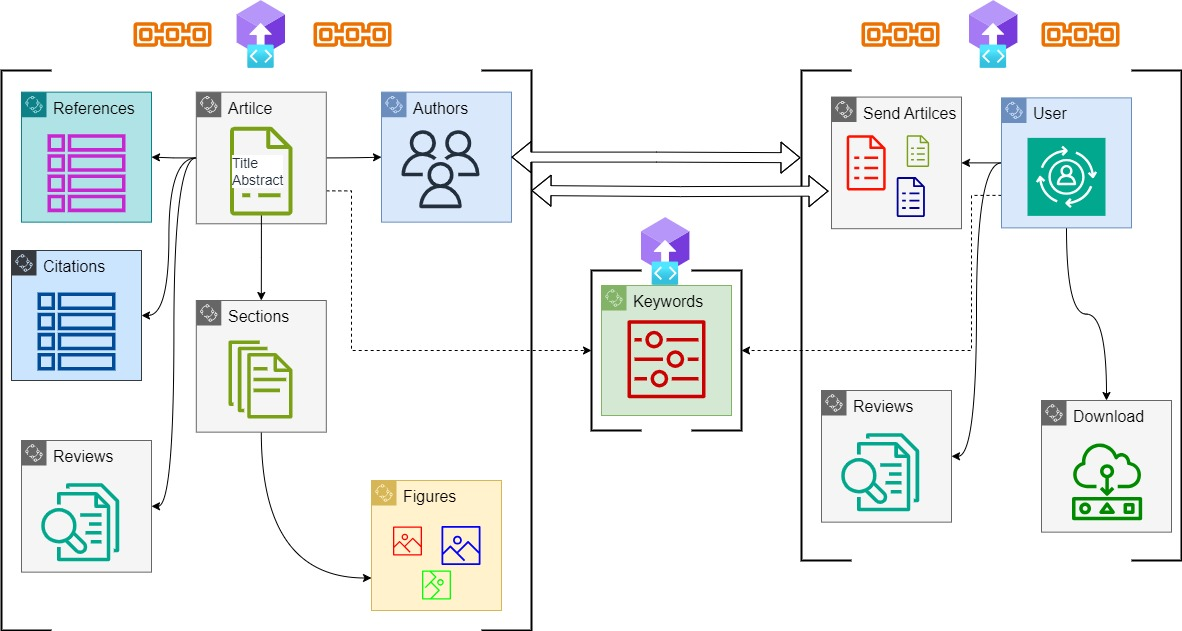
\includegraphics[width=\linewidth]{assets/inscription.jpg}
  \caption{Inscriptions of Article and User.}
  \label{fig:inscription}
\end{figure*}


Within the Journal DAO framework, each paper is stored in a blockchain block, which consists of multiple inscriptions. As illustrated in Figure \ref{fig:inscription}, the primary inscription records the paper's title and abstract, with sub-inscriptions(children) for the authors, keywords, figures, references, and detailed sections of the article. Once a paper enters the peer review process, the review outcomes are recorded as inscriptions on the blockchain (ensuring objectivity by making the review results visible while keeping the authors anonymous). After publication, the paper can be downloaded and cited by other users, further extending its blockchain record. The hierarchical relationship between parent and child inscriptions mirrors traditional academic paper management, creating a network structure of inter-referencing articles. However, due to the 4MB size limit of individual blockchain inscriptions, and given that many papers exceed this limit, recursive inscriptions are used to fully store papers on the blockchain, allowing the DAO system to achieve true decentralization. In Web 2.0 journal systems, there are primarily used for cross searching articles, but in a Web 3.0 journal system, recursive inscriptions also lay the foundation for decision-making processes and incentive mechanisms. Each user is represented by a profile composed of their research areas (keywords), published papers, and reviewed papers. Published papers, made up of inscriptions, feed back into the user's profile, capturing a wide range of influence factors, thus promoting deeper participation and recording more diverse contributions within the decentralized system \cite{BERTUCCI2024102338}.
% 在journal dao的框架中，一篇论文就在一个区块中，这个区块由多个铭文组成。如图2所示，文章的铭文记录了文章的标题以及摘要，此铭文的子铭文为：作者、关键字、图形、引用以及文章的详细章节。文章一旦进入了评审，会把评审的结果也记录在区块链的铭文中(为保障客观，文章的评审结果可见，作者不可见)；文章发布之后，它还会被别的用户下载，以及别的文章引用。文章铭文的父级与子级关系与传统的论文管理基本一致，会成为网状的结构，相互引用，但是在区块链中，因为单个铭文的大小限制为4MB，而一篇文章经常超过这个尺寸，使用递归铭文可以真正的把论文存于区块链中，让DAO系统真正的完成去中心化。文章内容相互引用，在web2.0杂志系统中，仅仅用来完成文章的交叉查询；但在web3.0杂志系统中，递归铭文，也给后面的决策部分以及激励机制创造了条件。每个用户也是由研究领域(关键字)，发表的文章，评审的文章组成的用户画像，尤其是发表的文章，本身就是铭文组成，又会反过来影响用户，尽可能多的记录了更多的影响因素。


In the practical implementation of the Journal DAO, this paper leveraged the Aragon framework to establish a decentralized and transparent infrastructure for academic publishing. The execution of the DAO involved several key steps to ensure a seamless and fair distribution of tokens among participants \cite{el2020overview}.
In a DAO, the concept of incentive mechanisms plays a crucial role in driving active participation and contributions. These mechanisms are designed to provide incentives and rewards to individuals or entities involved in the DAO's activities. By offering tangible benefits such as token rewards, governance rights, or recognition, participants are motivated to actively engage and contribute to the DAO's growth and development. Effective incentive mechanisms foster collaboration, maintain long-term motivation, and encourage innovation within the DAO community. The incentive design of journal dao promotes collaboration, maintains long-term incentives, and promotes innovation within the DAO community in the following aspects.
%在期刊 DAO 的实际实施中，我们利用 Aragon 框架建立了一个去中心化和透明的学术出版基础设施。 DAO 的执行涉及几个关键步骤，以确保代币在参与者之间的无缝和公正分配。
%在 DAO 中，激励机制的概念在推动积极参与和贡献方面发挥着至关重要的作用。这些机制旨在为参与 DAO 活动的个人或实体提供激励和奖励。通过提供代币奖励、治理权或认可等有形利益，参与者会被激励积极参与 DAO 的成长和发展并为其做出贡献。journal dao的激励设计在以下几个方面促进了协作、维护长期激励和促进DAO社区内的创新。

\begin{enumerate}
  \item Author motivations:
        %作者奖励：

        Authors, as the initial owners of the articles, receive a significant number of tokens at the beginning. Furthermore, they continue to earn tokens through article downloads and citations. The quantity of downloads and citations serves as an objective measure of the article's quality, showcasing its excellence. With more tokens, authors gain access to increased financial resources, which serves as motivation for them to produce better articles.

  \item Reviewer Incentives:
        %评审者激励：

        Reviewers are rewarded with tokens based on their contributions and responsibilities during the peer review process. Each time an article generates financial resources, reviewers receive their share based on their token holdings. This incentivizes more individuals to actively participate in the review process.

  \item Publisher rewards:
        %出版商：

        Publishers, being the providers of the entire journal system, initially receive the highest number of tokens, reflecting their responsibility for article publication. However, as articles are downloaded and cited multiple times, they will be surpassed by the author of the articles.

  \item Reader Bonuses:
        %读者奖金：

        Readers, when downloading and citing articles, also earn tokens. Although individual readers receive a smaller number of tokens, this opportunity allows them to generate income. This incentivizes readers to download and cite articles, and if the downloaded and cited article exhibit high quality, attracting more readers to engage with them, they can earn a substantial amount of financial resources.

\end{enumerate}

% 作者作为article的第一拥有人，初期就会获得较高的token，文章下载或者引用时候，又会持续获得token。下载引用的数量一般会客观证明论文有比较好的质量，证明了论文的优秀。拥有更多的token，也就拥有了更多的finance，这样会激励作者写出更好的文章。
% 评审者根据评审的贡献和责任获得token，每次文章创造了finance，评审者也都会根据自己持有的token获得相应的finance，这样会激励更多的人参与到评审过程中。
% 出版商是整个文章系统的提供者，并且要对article负责，在初期，理应获得最高的token。但是后续文章被多次下载以及引用时候，应该让利，被作者超过。
% 读者下载和引用论文时，也会获得token。虽然单个读者获得的token是最少的，但是给了读者赚钱的机会。会激励读者下载和引用论文，如果下载引用的论文有比较好的质量，越来越多的读者下载引用，也会获得相当客观的finance。





The workflow of the DAO, as shown in Figure \ref{fig:frameworkofblockchain} depicted. As the DAO initiates the token minting process, specific rules guide the allocation of tokens. Authors are categorized into corresponding roles such as corresponding author, first author, second author, and third author, and so on, each receiving a different token allocation based on their contributions and responsibilities within the manuscript. Similarly, reviewers play a crucial role in the token allocation process. Their allocation is determined by their role in the review process and the ratings they provide for the submitted manuscripts. The publisher, as the platform responsible for facilitating manuscript publication, also receives a certain allocation of tokens due to their administrative role in managing the manuscripts.

This meticulous token allocation mechanism ensures that each contributor, be it an author or a reviewer, receives fair rewards based on their specific contributions and responsibilities \cite{10123021}. By implementing such a structured system, the DAO creates a transparent and equitable environment, aligning the incentives for authors and reviewers. This not only cultivates a sense of fairness within the system but also encourages active and meaningful participation from all parties. Guided by DAO principles, the workflow fosters seamless integration of all stakeholders, ensuring a well-functioning and self-sustaining ecosystem.
%在图示的工作流程中，流程始于用户提交论文进行出版。随着DAO启动铸币过程，特定规则指导着代币的分配。作者根据其在论文中的角色分为通讯作者、第一作者、第二作者和第三作者，每个人按照贡献和责任都获得不同的代币分配。同时，审稿人在代币分配中发挥着至关重要的作用。他们的分配由他们在审稿过程中的角色和对提交的论文的评分决定。出版商作为提供论文发布的平台，又有管理论文的职责，也分配了一定的代币。这种细致入微的代币分配机制确保了每个贡献者，无论是作者还是审稿人，都能根据其具体的贡献和责任公正获得奖励。通过实施这样一个结构化的系统，DAO创造了一个透明而公平的环境，使作者和审稿人的激励保持一致。这不仅在系统内部培养了公正感，还鼓励各方积极而有意义地参与。受DAO原则指导的工作流程促进了各利益相关方的无缝整合，确保了一个运行良好且自我维持的生态系统。




Every participant in the system has a specific number of tokens by contribution, then finance distributed according to the number of tokens. In this system, authors, reviewers, publisher, readers(who download the papers or references) all possess a specific quantity of tokens. These tokens are considered as NFTs due to their unique nature. Once finance is generated, the system allocates this finance based on the number of tokens held by the respective parties.This design ensures objectivity, fairness, and transparency within the system. Each participant's contribution is reflected in a specific number of tokens, and the allocation mechanism operates according to the quantity of these tokens. Such a design not only enhances the fairness of the incentive mechanism but also makes the entire system more transparent, allowing participants to clearly understand the relationship between their contributions and rewards.This NFT-based token system provides tangible and verifiable returns for contributors while establishing an effective and operable incentive mechanism for the entire ecosystem \cite{kong2021alternative}. This fair and transparent allocation method is expected to drive collaboration and development in the academic community, creating a mutually beneficial environment for all stakeholders.

%在这个系统中，作者、审稿人、下载用户和引用用户都拥有一定数量的token。这些token具有唯一性，可以被视为NFT（非同质化代币）。一旦产生了finance，系统会按照持有者的token数量来分配这部分finance。这个设计确保了系统的客观性、公正性和透明性。每个参与者的贡献都以特定数量的token体现，而分配机制则按照这些token的数量来进行。这样的设计不仅提高了激励机制的公正性，也使得整个系统更加透明，参与者可以清晰地了解他们的贡献与奖励之间的关系。这种以NFT为基础的token系统为贡献者提供了具体的、可证明的回报，同时也为整个生态系统提供了一种有效的、可操作的激励机制。这种公正而透明的分配方式有望推动学术界的合作与发展，为各方创造一个共赢的环境。



\subsection{The Advantages}




\begin{figure}[h!]
  \centering
  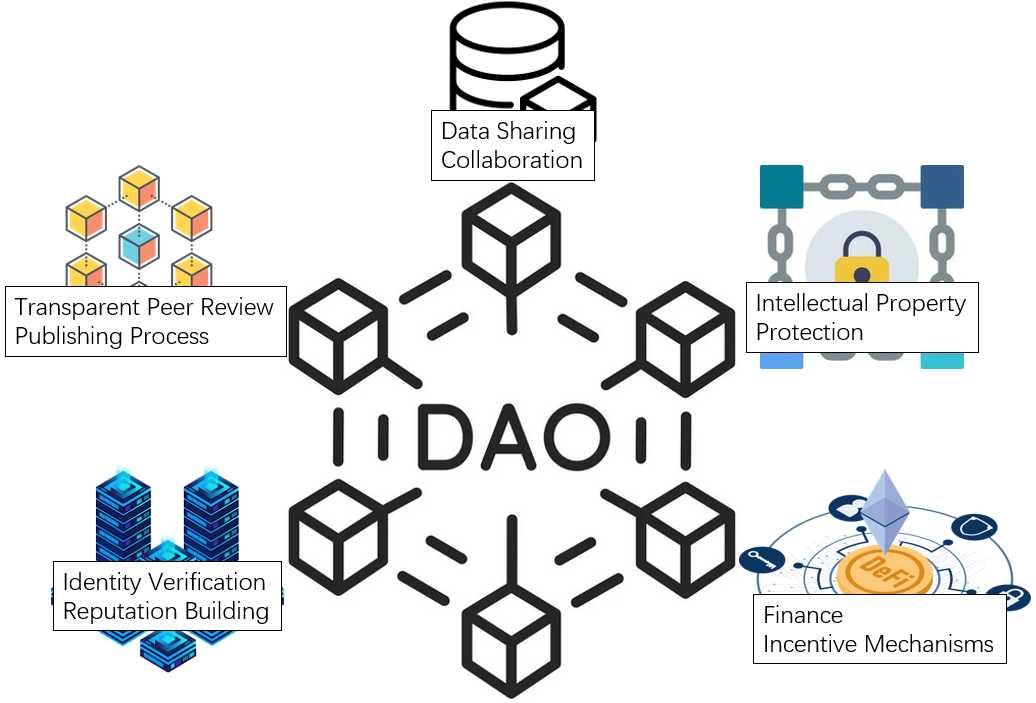
\includegraphics[width=\linewidth]{assets/dao.png}
  \caption{Application of DAO in Article and Journal}
  \label{fig:applicationofdao}
\end{figure}
% change3 更换图，改成web2跟web3的对比

According to the development of district DAO, related blockchain technology, the following DAO to Decentralized Science (DeSci) framework can be summarized as shown in the figure \ref{fig:applicationofdao}.It aims to establish a decentralized scientific publishing platform using blockchain and smart contract technology, enabling fair, transparent, and efficient scientific research dissemination.
%按照区DAO，以及相关区块链技术的发展，可以如图总结出以下的DAO框架。它旨在通过区块链和智能合约技术，建立一个去中心化的科学出版平台，实现科学研究的公平、透明和高效。

\begin{itemize}
  \item \textbf{Transparent Peer Review and Publishing Process:}

        Blockchain can be used to create a transparent academic publishing platform, ensuring transparency throughout the peer-review and publishing processes.\cite{nakamoto2008bitcoin} Smart contracts can manage review, publication, and payment procedures, ensuring traceability and fairness.
        %透明的学术出版： 区块链可以用于创建透明的学术出版平台，确保审稿和出版过程的透明性。智能合约可以管理审稿、出版和付款流程，确保可追溯和公平。

  \item \textbf{Protection of Intellectual Property:}

        Blockchain and smart contracts can safeguard authors' intellectual property, ensuring their works are not copied or distributed without permission \cite{gurkaynak2018intellectual}.
        %知识产权保护： 区块链和智能合约可用于保护作者的知识产权，确保其作品不会未经许可就被复制或传播。

  \item \textbf{Identity Verification and Reputation Building:}

        Blockchain can be employed to establish scholars' identities and reputations \cite{radziwill2018blockchain}. Smart contracts can automate the validation of scholars' achievements, storing them on the blockchain.
        %身份验证和声誉建立： 区块链可用于建立学者的身份和声誉。智能合约可以自动化验证学者的成就，并将其存储在区块链上。

  \item \textbf{Data Sharing and Collaboration:}

        Blockchain and smart contracts can facilitate data sharing and collaboration among scholars, ensuring data integrity and traceability \cite{praitheeshan2019security}.
        %数据共享和合作： 区块链和智能合约可用于促进学者之间的数据共享和合作，确保数据的完整性和来源可追溯。

  \item \textbf{Finance and Incentive Mechanisms:}

        DAO and cryptocurrencies can be used to support research finance and incentive mechanisms.Funds can be allocated according to token weights \cite{schar2021decentralized}.
        %金融和激励机制： 区块链和加密货币可以用于支持学术研究的融资和激励机制。资金可以按照token为权重分配。
\end{itemize}

These application examples highlight the potential value of blockchain, smart contracts, and DAO technology in academic publishing and journal management. They enhance transparency, protect intellectual property, verify identity, automate processes, and encourage collaboration. As these technologies continue to evolve, they hold promise for further innovation and efficiency in academia \cite{vacca2021systematic}.
%这些应用示例突显了区块链、智能合约和DAO技术在学术出版和杂志管理方面的潜在应用，提高了透明度、知识产权保护、身份验证和自动化审稿流程。随着这些技术的不断发展，它们将有望为学术界提供更多的创新和效率。


In the current web2.0 landscape, both literature storage and payment systems are typically centralized, controlled by a single entity or organization. However, in the decentralized web3.0 network, article data resides directly on the blockchain \cite{alabdulwahhab2018web}, with websites serving as interfaces to access this data \cite{10402553} \cite{971982} \cite{6222336}.
In this new framework, payments are automated and executed through smart contracts within the DAO framework \cite{cao2022decentralized}. This ensures complete transparency and traceability, as the fund distribution process follows predefined rules without centralized supervision \cite{10302676}.
In the Web 3.0 paradigm, this novel model signifies a departure from reliance on traditional intermediaries. Instead, it empowers users with the direct participation in DAO frameworks, utilizing smart contracts for automated and secure fund distribution \cite{10302435}. This shift not only achieves decentralization in the transaction process but also enhances the efficiency of academic article transactions.
In the Web 3.0 environment, articles are directly uploaded to the blockchain. All operations, including payment processing and fund distribution, are seamlessly executed through smart contracts.
% 在当今web2.0的下，无论文献的储存或者支付系统，通常都是集中式的，这意味着它们由单个实体或组织控制。在去中心化网络的web3.0，文章数据主体直接存在于区块链上，而网站仅仅是对区块链数据的映射。在这一新的框架下，整个资金分配的过程都通过智能合约进行自动化执行，无需手动干预。这一创新性框架确保了整个过程的完全透明性和可追溯性。当用户支付下载文章时，资金会根据去中心化自治组织（DAO）框架内设立的规则自动分配，无需任何集中监管。
%在Web 3.0的范式中，这一新兴模式标志着我们不再依赖传统中介机构。相反，它赋予用户直接参与DAO框架的权力，利用智能合约实现资金的自动化和安全分配。这一转变不仅实现了交易过程的去中心化，还提高了学术文章交易的效率。
%在Web 3.0的环境中，文章直接上链。所有操作，包括支付处理和资金分配，都通过智能合约无缝执行。

\section{Mechanism Design of Journal DAO \label{sec:mechanism}}
% \section{Mechanism Design of Journal DAO \label{sec:mechanism}}本节共2页
% 简要写一下本节的思路，3-5行即可。

% \subsection{Decentralized Governance}

% \subsection{Initial Token Distributions}

% \subsection{Token Distributions upon Article Download or Citation}

% \subsection{Finance Distributions}

%【本节是最重要的部分，一定要体现创新性，想一想在机制设计的过程中，哪里可以有一些创新】


% 开头1小段介绍本节要做什么。


% A.治理机制？


% B.代币分配机制


% C.Finance分配机制


% 本节是介绍具体的机制设计过程，要详细，不是像A部分那样笼统地说





% 本文结合DAO的基本概念，创建DAO的框架。首先是铸币，其中为所有与论文相关的参与者，包括审稿人，作者，读者，按照一定的机制分配token。token可以用来决定proposal的权重，本框架根据token分配finance。


% This paper combines the fundamental concepts of DAO to establish a framework for implementing DAO in academic journals. The framework begins with the issuance of tokens, which are allocated to all participants involved in the publication process, including reviewers, authors, and readers, through a specified mechanism. These tokens serve as a means to determine the weightage of proposals, and the framework utilizes the token distribution to allocate financial resources accordingly. By integrating token-based incentives and governance mechanisms, this framework ensures a fair and transparent distribution of resources within the DAO-operated journal ecosystem. Participants holding tokens can actively participate in the processes of all aspects of the article publication, such as send articles, review articles, and download articles, thereby influencing the allocation of financial resources based on their token holdings. Through this framework, the DAO-operated journal can foster an inclusive and democratic environment, empowering participants to shape the direction and priorities of the journal based on their token weightage.
This paper introduces a DAO framework tailored for academic journals, incorporating fundamental concepts of DAO to achieve autonomy within the organization. By implementing effective incentive mechanisms, the framework enables fair and autonomous governance. The framework initiates the minting process, wherein tokens are allocated to all participants involved in the scholarly publication process, including reviewers, authors, and readers, based on predefined mechanisms. These tokens hold the power to influence proposal weighting, and allocates financial resources according to token distribution.
The application of blockchain technology ensures equitable and transparent resource allocation within the scholarly journal ecosystem. Participants holding tokens actively engage in the article publication process, such as submitting articles, reviewing papers, and downloading research outputs, thereby influencing the distribution of financial resources based on their token holdings. Through this framework, academic journals operated by DAOs can foster an inclusive and democratic environment, prioritizing the interests of all stakeholders involved.
By combining the principles of DAO with academic journal operations, this framework paves the way for a decentralized and community-driven approach to scholarly publishing \cite{10426804}. It empowers participants, promotes collaboration, and ensures the fair distribution of resources, ultimately leading to a more inclusive and sustainable academic publishing ecosystem.
%本文结合DAO的基本概念，创建了一个适用于学术期刊的DAO框架，使用有效的激励机制，让整个机构实现自治。该框架首先进行铸币操作，将与论文相关的所有参与者（包括审稿人、作者和读者）按照一定的机制分配代币。这些代币可以用来决定提案的权重，也能根据代币分配finance资源。区块链技术的应用，使该框架下的学术期刊生态系统中的资源公平和透明分配。持有代币的参与者可以积极参与文章发布过程，例如发布文章、审阅文章和下载文章，从而根据其代币持有量影响财务资源的分配。通过该框架，DAO运营的学术期刊能够营造一个包容和民主的环境，最重要可以给所有参与者相应的利益。

%



In this DAO framework, token distribution is determined by a formula that takes into account the token holdings of different participants. As Equation \ref{eq:dao} denote the token holdings of authors, reviewers, publishers, and readers as $A$, $E$, $P$, and $R$, respectively. The allocation mechanism, represented by the variable $\omega$, calculates the total token holdings after each event, denoted as the sum of token changes over a given period $(t)$.


\begin{equation}
  \begin{bmatrix}
    A_t \\
    E_t \\
    P_t \\
    R_t
  \end{bmatrix}
  =
  \omega_{t-1}
  \begin{bmatrix}
    A_{t-1} \\
    E_{t-1} \\
    P_{t-1} \\
    R_{t-1}
  \end{bmatrix}
  +
  \omega_{t-2}
  \begin{bmatrix}
    A_{t-2} \\
    E_{t-2} \\
    p_{t-2} \\
    R_{t-2}
  \end{bmatrix}
  +
  \cdot
  +
  \omega_n
  \begin{bmatrix}
    A_n \\
    E_n \\
    P_n \\
    R_n
  \end{bmatrix}
  \label{eq:dao}
\end{equation}



The variable $\omega$ represents the weight assigned to each event, indicating the impact of that event on token changes. This weight can be adjusted based on specific criteria, such as the quality of the article, the level of contribution by reviewers, or the number of downloads and citations by readers.
By incorporating this formula into the DAO framework, token distribution becomes a dynamic process that reflects the contributions and activities of all participants.
% 公式1中，A代表了作者的token持有量，E代表了审稿人的token持有量，P代表了出版商的token持有量，R代表了读者的token持有量。w代表了分配机制，最终的token持有量为所有的t次事件造成的token改变的总和。



\subsection{Decentralized Governance}
%去中心化治理：

% 重新画图。作者的发文章，以及改完整全都在一个去中心化的流程上。审稿人的安排，以及审稿也都是在去中心化的流程上。对比之前的web2,虽然评审的过程是匿名的，但是是否匿名完全靠对出版商的信任，去中心化可以保证投稿和审稿的过程都是匿名的，基本去除了人为的主观意见。

% 去中心化决议，审稿的过程，与DAO的投票决议基本吻合。传统的审稿，需要EIC分配SE以及AE，还要指定一定数量的Reviewer，各种操作比较集中。去中心化的审稿中，根据


% 递归铭文在审稿中的应用：每一个审稿人拥有多个属性，多个属性以递归铭文的方式组成了一个审稿人的数字画像。此种方式在减少了数据承载量，并更直观的显示出了每个审稿人的特征。在分配审稿人时候，可以按照这个特种更有效的分配审稿人。并且以铭文在文章中的占比，动态的决定了审稿人的权重。


DAO, adopting a decentralized governance model, allows token holders to participate in the decision-making process. This ensures community involvement in platform development, creating a democratic and inclusive environment. With robust incentives in place, token holders have made outstanding contributions while also receiving greater rewards. This positive feedback loop forms a self-sustaining ecosystem of active governance \cite{beck2018governance}. DAOs leverage blockchain technology to provide transparency and trust, recording all proposals, votes, and transactions on the blockchain for public verification. Incentives motivate token holders to actively engage in the governance process, while DAOs offer a meritocratic approach that values expertise. The flexibility and adaptability of DAOs allow them to evolve and respond to the needs of the community. However, challenges such as active participation, governance gridlocks, and power concentration need to be addressed through clear rules and mechanisms. Overall, DAOs empower token holders, foster community involvement, and create a democratic and inclusive environment \cite{jensen2019theory}.
%DAO采用去中心化治理模型，允许代币持有者参与决策过程。这确保了社区能够参与平台发展，创造了一个民主和包容的环境。在比较优秀的激励下，代币持有者做了出色的贡献，同时也获得更多的奖励。一个积极的自治体系完美闭环。DAO借助区块链技术提供透明度和信任度，将所有提案、投票和交易记录在区块链上，供公众验证。激励机制激励代币持有者积极参与治理过程，而DAO则提供了重视专业知识的优秀人才的机会。DAO的灵活性和适应性使其能够随着社区的需求而发展和应对变化。然而，需要通过明确的规则和机制来解决积极参与、治理僵局和权力集中等挑战。总体而言，DAO赋予代币持有者权力，促进社区参与，并创造民主和包容的环境。

\begin{figure}[h!]
  \centering
  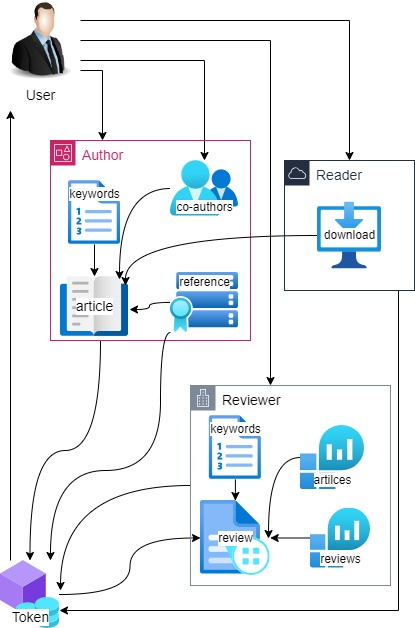
\includegraphics[width=\linewidth]{assets/govern.jpg}
  \caption{User got Tokens by Roles.}
  \label{fig:userRoles}
\end{figure}


In the Journal DAO framework as illustrated in Figure \ref{fig:userRoles}, after articles are divided into recursive inscriptions, each inscription is assigned a specific weight. During token minting events, tokens are distributed based on these weights, and these tokens will generate future finance. As authors, including co-authors or corresponding authors, users receive a certain amount of tokens when publishing an article. However, the number of tokens is influenced by factors such as co-authors, keywords, and cited references. For reviewers, their previous reviews increase the weight of their expertise in a particular research area, and their previously published articles also contribute to this weight. This weight affects their influence during the review process, which in turn impacts their token rewards. Even readers can earn tokens; whether through individual paid downloads or institutional access, a small portion of tokens is allocated based on the weight of the article’s inscriptions. Additionally, by downloading an article, users influence its weight, thus participating in decision-making and earning rewards. Through this system, all participants—authors, reviewers, and readers—are incentivized to engage with the framework, creating a decentralized, self-sustaining ecosystem.
% 用户用递归铭文划分之后，每一个铭文都是一个权重，在铸币事件的时候，会按照权重分配相应的token,这些token日后都会创造收益。用户作为作者(二作或者通讯作者)，每次发布文章的时候，都会获得一定数量的token，token的数量会被其他作者、关键字、引用文献影响。用户作为审稿人，之前的审稿会给自己研究的领域增加权重，之前发布的文章也会同样影响，这个权重会影响自己评审时决策的占比，这个占比又会反过来影响token的获得。用户甚至作为读者都会获得收益，不管用户个人知识付费下载论文，还是用机构下载论文，也都会按照权重分配少量的token，(用户下载同样也会影响文章)，自己也会参与到决策中，也会获得收益。



The implementation of the Journal DAO has yielded positive results in terms of increased engagement, quality submissions, and a more inclusive academic ecosystem. The transparent and automated token distribution mechanisms have effectively addressed issues of ownership and reward distribution, fostering a collaborative and fair scholarly environment.
In order to create a strong incentive for active participation, a well-designed incentive mechanism is implemented in the decentralized governance framework. After authors publish their articles, the generated finance from user downloads is distributed not only to the publishers but also to all the authors and reviewers, motivating authors to produce high-quality articles and encouraging more individuals to serve as reviewers.
To further enhance participation, readers who download the papers are also allocated a share of the revenue. This encourages more people to download the papers, leading to increased revenue for the DAO. As a result, all participants are incentivized to actively engage in the ecosystem, fostering a thriving and automatic academic community.
This incentive mechanism ensures that all contributors, including authors, reviewers, publishers, and readers, are fairly rewarded for their contributions. It creates a positive cycle where authors are motivated to produce quality work, reviewers are incentivized to provide valuable feedback, and readers are incentivized to access and support the academic content. Overall, this system promotes a healthy and autonomous academic ecosystem within the DAO framework \cite{bolton1998corporate}.
%期刊 DAO 的实施在提高参与度、质量投稿以及创建更具包容性的学术生态方面取得了积极成果。透明和自动化的代币分配机制有效解决了所有权和奖励分配的问题，促进了合作和公正的学术环境。
% 是用一个比较好的激励机制，让所有参与者都能积极参与。作者发表论文之后，用户下载时创造的finance除了给出版商外，所有的作者以及审稿人都可以分得收益，会让作者更有写作优秀文章的动力；审稿人也会获得收益，会有更多的人愿意做审稿人。现在，给下载论文的读者也分配收益，会有更多的人愿意下载论文，有更多的人下载论文，DAO就会有更多收益，这样就能让所有的参与者都能积极参与，形成一个良好的自治学术生态。

\subsection{Initial Token Distributions}


% DAO 框架中，token是至关重要的部分，它决定了决策成功的占比，更在财务分配时候决定了比例。token的生产，称之为铸币，一般会有多次铸币，一些行为都会影响token的分配数量。

\begin{figure}[h!]
  \centering
  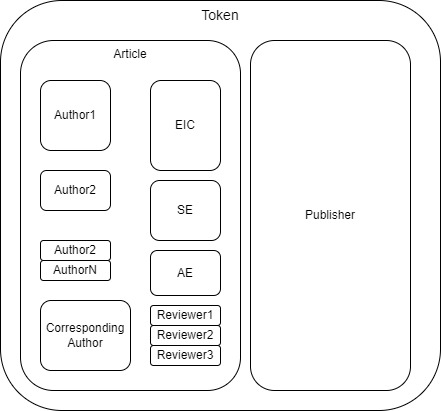
\includegraphics[width=\linewidth]{assets/initialmint.jpg}
  \caption{Initial Token Distribution.}
  \label{fig:initialmint}
\end{figure}

In this framework as illustrated in Figure \ref{fig:initialmint}, the publication of a article creates a small ecosystem. At the time of creation, the initial token minting is substantial, involving three key groups: authors, reviewers, and the publisher. Tokens are distributed among these groups based on predefined proportions that reflect their responsibilities. Since there is typically only one publisher, their portion is straightforward. An article usually involves multiple authors, each receiving a share based on their role, with the first author and corresponding author typically receiving a larger portion. Each author’s contribution is further broken down into multiple inscriptions, allowing for adjustments to the allocation based on the weight of these inscriptions. During the review process, multiple reviewers are involved, and each reviewer is assigned a proportion of tokens based on their role. This system ensures that all authors, reviewers, and the publisher are fairly compensated, creating a balanced and transparent token distribution model.
% 在本框架中，一篇论文的发表就创建了一个小的生态。创建时候的第一次铸币量非常大，其中包括了作者，审稿人，出版商。这三个群体中，按照责任制定了比例，token会按照这个比例分配。出版商只有一个，不多赘述。一篇文章，一般是由多个作者组成，每个作者都有自己的比例，比如一作和通讯作者会占比多一些。一个作者是由多个铭文组成，根据铭文又可以对占比做出一定的调整。文章在审稿过程中，会有多个审稿人，每个审稿人都有自己的比例。

In this framework, reviewer tokens play a crucial dual role, both influencing decision-making during the review process and determining financial compensation. In traditional journal systems, reviewers are selected based on their research areas, then ensuring that no reviewers come from the same institution, and adhering to certain quantity requirements, such as needing a minimum number of reviewers before an AE can pass their recommendations to a SE or EIC. The DAO framework adopts these practices—assigning reviewers based on their research fields and avoiding conflicts of interest with institutions—while making the process more transparent. In the DAO system, reviewer assignments are not only governed by quantity but also by token limitations. Typically, the framework requires a minimum token threshold to be reached for any decision to move forward. Only after this threshold is met can voting take place, with the proportion of tokens influencing the final decision. This token-driven, decentralized decision-making process ensures that peer review becomes more authentic, transparent, and accountable, addressing many of the inefficiencies and opacity present in traditional systems.
% 本框架分配了审稿人token，这个token即在审稿决策时候起到了关键作用，又在财务分配时候决定了其收入。传统的杂志系统，分配审稿人时候，首先可以参考审稿人的研究领域，然后是避免相同机构审稿，最后是数量要求，比如要求至少一定数量的审稿人完成审稿，AE才能继续审稿给SE以及EIC提交审稿意见。DAO框架中，按照审稿人的研究领域进行分配，以及避免相同机构审稿都会沿用，并且会更透明。审稿那部分不只是按照数量会按照审稿人的token限定，一般DAO框架中都会要求一个决议至少总参与人凑够多少token才能通过，然后才是投票时候按照比例决定是否通过。使用DAO完成决策会让审稿流程变得更加真实，更加透明。



In a DAO framework, decision-making regarding financial allocation. By employing token allocation based on NFT principles, the framework ensures a fair distribution of rewards among token holders. Through transparent smart contracts, the DAO framework establishes a self-regulating environment that incentivizes active participation and contribution. The implementation of this token-based distribution mechanism requires tracking token ownership and automated distribution of finance.
% 在DAO框架下，一个决策可能是分配finance，按照nft的方式，把token作为分配的比例，一旦产生了finance，就按照所有holder都可以按照比分到finance。

\begin{equation}
  \begin{aligned}
    T   & = A + E + P                                                \\
        & (A=\{a_{corresponding}, a_1, a_2, a_3, \cdots a_n\})       \\
        & (E=\{e_{EIC}, e_{SE}, e_{AE}, e_1, e_2, e_3, \cdots e_m\}) \\
        & (P=\{p\})                                                  \\
    F   & \in \{ ETH, Bitcoin, \cdots \}                             \\
    a_1 & = F \frac{T_{a_1}}{T}                                      \\
    e_1 & = F \frac{T_{e_1}}{T}                                      \\
  \end{aligned}
  \label{eq:finance}
\end{equation}


According to equation \ref{eq:finance}, the total number of tokens is denoted by $T$, and the token distribution for authors, reviewers, and publishers is represented by $A$, $E$, and $P$, respectively. Here, $A$ represents the set of all authors, including the corresponding author; $E$ represents the set of all reviewers, including the EIC, SE, and AE; $P$ represents the publisher. Once finance, denoted as $F$ (which could be in the form of ETH, Bitcoin, or other cryptocurrencies), it is distributed among all token holders proportionally to their token share. For example, the first author of a paper will receive a share of the finance proportional to their token allocation divided by the total tokens. As long as a user holds tokens, they are entitled to a portion of the finance. Since tokens not only determine decision-making power but also govern future income, this system strongly incentivizes users to actively participate in both submitting papers and reviewing them, as their involvement directly influences their token allocation and, consequently, their financial rewards.
% 根据公式\ref{eq:finance}，总共的token是$T$ 作者、审稿人、出版商的token分配为$A$, $E$, $P$，A为所有作者的集合，包含通讯作者，E为所有审稿人的集合包括EIC、SE、AE，P为出版商。一旦产生finance,$F$为finance可能是ETH、Bitcoin等，会按照这个比例分给所有holder，比如文章的一作，分的比例为自己的token比上所有的token，只要有token就会分得finance。因为token除了确定决策权，还决定了以后的收入，在这个环境下，用户会更积极的完成投稿以及审稿。



\subsection{Token Distributions upon Article Download or Citation}

% change 7 这块减少描述，最好改成闭环的建议

Paid knowledge access has existed for a long time, with many journals offering paid downloads of articles, either through individual or institutional payment models. Download and citation counts are key metrics for evaluating the impact of an article, and within the recursive inscription structure of the article, these metrics are critical indicators. In the current framework, each download event also triggers a token-minting event. In addition to proportionally distributing tokens to the authors, a portion of tokens is also allocated to the downloader. Downloading an article signifies recognition of the work and its authors, so it is appropriate that tokens are distributed to the authors. At the same time, since the downloader, as a reader, has contributed to the article's visibility and impact, it is justifiable that they receive tokens as well, reflecting their role in contributing to the article’s overall value.
% 知识付费，很早就有，很多杂志都有付费下载论文的功能，有个人付费，也有机构付费。论文的下载量和引用量是评价一个论文的重要指标，所以在组成文章的递归铭文中，下载量和引用量是一个重要的指标。当前框架中，在文章的下载也创建了一个铸币事件，除了按照比例给作者分配token外，还会给下载者分配比例的token。下载论文，是对文章的认可，也是对文章作者的认可，所以token需要分给作者，用户作为读者认可了这篇文章，也是给了文章贡献，获得token也天经地义。


\begin{figure}[ht]
  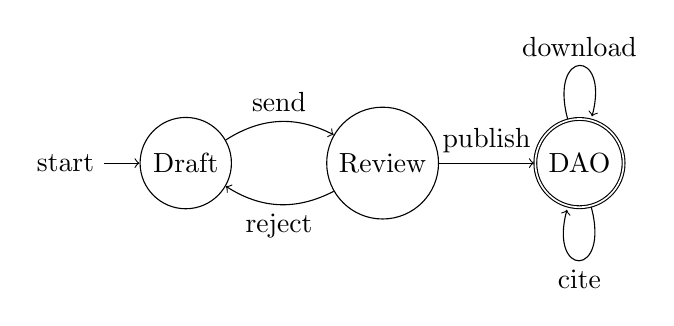
\begin{tikzpicture}[node distance=2.5cm, on grid]
    \node[state, initial] (q1) {Draft};
    \node[state, right=of q1] (q2) {Review};
    \node[state, accepting, right=of q2] (q3) {DAO};

    \path[->]
    (q1) edge[bend left, above] node {send} (q2)
    (q2) edge[bend left, below] node {reject} (q1)
    (q2) edge[left, above] node {publish} (q3)
    (q3) edge[loop above] node {download} (q3)
    (q3) edge[loop below] node {cite} (q3);
  \end{tikzpicture}
  \caption{Automata Machine of the Framework}
  \label{fig:automataMachine}
\end{figure}

Compared to the article's authors, the contribution of downloaders is minimal, so the tokens they receive are proportionally fewer. As illustrated in the automaton in Figure \ref{fig:automataMachine}, the token minting event triggered by publishing an article is a one-time occurrence. However, the token minting from downloads happens repeatedly. In the ecosystem of an article, citations also generate recurring token minting events. For a high-quality article, there can be an unlimited number of downloads and citations, leading to an ever-increasing accumulation of tokens for the authors. As authors continue to earn more tokens, their influence in decision-making within their research field grows, as their token holdings grant them greater voting power in governance decisions. Additionally, their share of finance within the framework increases proportionally, offering significant financial incentives over time. Each download event represents a finance-generating action, and before tokens are distributed, the download finance is proportionally allocated to all stakeholders. This includes all authors, reviewers, publishers, and even readers who have previously downloaded the paper. This cyclical and continuous distribution mechanism ensures that all contributors, from creation to consumption, are rewarded fairly, while authors of impactful work benefit the most.
% 相比于文章的作者，下载者的贡献非常小，所以获得toekn非常少。在一篇文章的生态下，如图1的自动机，发布论文的铸币，是唯一一次获得token的事件。但是下载论文的铸币，是多次获得token的事件。发布文章，引用这篇文章在这篇文章的生态下，也是多次的循环铸币事件。对于优秀的文章，会有无限多次的下载和引用，作者获得token也会越来越多，作为文章作者的用户，拥有更多的token，在其研究领域的决议占比会更高，并且获得finance也会越来越多。下载论文是有finance的事件，分配token之前，会按照比例把下载的收入分给所有holder，其中有所有作者、所有审稿人、出版商，甚至还有下载过这篇文章的读者。




\begin{equation}
  \begin{aligned}
    F_{r}^*  & = \sum_{i=0}^{n} F_{ei} \frac{T_{r}}{\sum_{j=0}^{i}T_j}           \\
    \omega_r & = \frac{F_{r}^*}{F_{e}} = \sum_{i=0}^{n} \frac{T_{r}}{T_0 + iT_1} \\
    \omega_r & = \sum_{i = 1}^{n} \frac{1}{W_0 + i W_1}
  \end{aligned}
  \label{eq:breakeven}
\end{equation}

As readers, users currently receive minimal rewards but they contributing real financial resources. Implementing a more effective incentive mechanism that allows users to break even or potentially earn more than they spend would not only encourage greater participation but also promote the autonomy of the DAO. Such a system would reinforce the value of knowledge and contribute meaningfully to the concept of paid knowledge. By aligning incentives with user contributions, this approach would drive more active engagement and strengthen the overall sustainability of the knowledge economy within the DAO framework.
% 用户作为读者的收益非常小，但是他们是真的付出了finance，此处，如果有个比较好的激励机制让用户可以收入跟支出持平，甚至有的赚，会促进DAO的自治，甚至为知识付费贡献了一份力量。

According to Equation \ref{eq:breakeven}, the total income for readers who download articles within the DAO framework is denoted as $F_{r}^*$. Each download generates a financial gain, $F_{e}$, which is distributed among all token holders based on their respective token proportions. The reader's income from a specific download is represented as $F_{en} \frac{T_{r}}{\sum_{i=0}^{n}T_i}$. As other readers download articles more frequently, the total token holdings within the system gradually increase. Thus, while the reader's income may increase over time, the income from each individual download decreases.
The finance received from each download event is fixed. By comparing the reader's total income with their expenses, which is equivalent to the finance per download event, a ratio called $\omega_r$ is obtained. When this ratio equals 1, the reader's income matches their expenses, and any subsequent income becomes additional. $T_r$ represents the number of tokens held by the reader and remains constant. To simplify the equation, $T_0$ and $T_1$ are expressed as ratios to $T_r$, denoted as $W_0$ and $W_1$, respectively. Ultimately, the balance between income and expenses is determined by $W_0$, and $W_1$,.
% 按照公式9所示，Fr为DAO中，下载了article的读者的总收入。每一次下载，都会有Fe的finance进账，然后会按照token的比例分给所有的holder，读者本次的收入就是Wr。因为读者的贡献只有下载article那一次事件，所以token不会增加，但是随着别的读者下载论文次数越来越多，总token会越来越多，所以虽然读者的收入是逐渐增高的，但是每次都收入是逐渐减少的。每次下载论文的finance是固定的，现在把读者的总收入，比上用户自己下载论文时候的花销，也就是以后每次下载论文的finance，得到一个比例omega，当这个值为1时候，读者的收入跟复出持平，之后的收入全都是额外收入。Tr作为读者持有的token数，值不会改变，所以缩减此变量，T0和T1变成跟Tr的比例，W0和W1。最后可以明确表示收支平衡由W0和W1决定。


\begin{equation}
  \begin{aligned}
    \omega_r^1 & = \sum_{i = 2}^{n} \frac{1}{W_0 + i W_1}     \\
    \omega_r^t & = \sum_{i = t + 1}^{n} \frac{1}{W_0 + i W_1}
  \end{aligned}
  \label{eq:evenotherreader}
\end{equation}



However, to prevent users from simply following trends, it is essential to implement mechanisms ensuring that users genuinely value the articles before earning rewards. In the context of Equation \ref{eq:evenotherreader}, the allocation of financial gain within the DAO framework is elucidated. The first reader who downloads the article obtains the entirety of the financial gain from all subsequent events. However, subsequent readers can only receive their share of the financial gain starting from the next download event. For instance, the second reader can obtain finance only from the second download event onwards, and the $t$-th reader can receive finance from the $t+1$-th download event.
This allocation mechanism is influenced by the continuous increase in the total quantity of tokens within the DAO system. Consequently, earlier events hold a higher proportion of the financial gain, while later events receive a smaller portion. As each download event yields a gradually diminishing income, waiting for a high download count before downloading the article may result in an inability to reach a break-even point, where income matches expenses.
% 但是要防止用户跟风，所以要限制必须用户自己真的认可了文章，才能获得收益额。根据公式10所示，第一个下载article的读者，可以分得全部事件的finance。第二个下载的读者，就要从下一个下载事件才能分得finance，第二t个，从第t+1个下载才能分得finance。因为DAO的token总量在持续增加，所以越早的事件，分得的finance越多，越晚分得的越少。因为每一次都收入是逐渐减少的，所以论文一旦下载量比较高时候再下载，可能永远不会跟支出持平。


\section{A Case Study \label{sec:performance}}

In this section, we present experimental results by adjusting several parameters to reasonable values and conducting experiments to observe the distribution of the results. These experiments aim to provide insights into the outcomes under different parameter settings and offer a better understanding of the system dynamics. By analyzing the experimental results, we can evaluate the impact of parameter adjustments on the observed distributions, enabling us to make informed decisions and recommendations for optimizing the system performance.
% 本节给出一些实验结果，调整相对合理的一些参数，然后进行实验，观察实验结果的分布。

\subsection{ Parameters Adjust and Simulation}

According to Equation \ref{eq:breakeven}, the factors influencing the balance between income and expenses are represented by $W_0$ and $W_1$. To visualize these factors, we will now construct a heatmap. The value of $W_0$ is expected to be relatively large as it encompasses the major contributors within the current DAO, such as authors, reviewers, and publishers. On the other hand, the value of $W_1$ is expected to be relatively small and involves only authors and readers, but it continues to cycle and trigger recurrently.
% 根据公式9，影响收支平衡率的因素，为w0和w1，现在绘制热力图。w0的值理应比较大，因为包含了当前DAO中贡献最大的作者，审稿人，以及出版商。w1的值理应比较小，并且只包含作者和读者，但是会一直循环触发。

\begin{figure}[h]
  \centering
  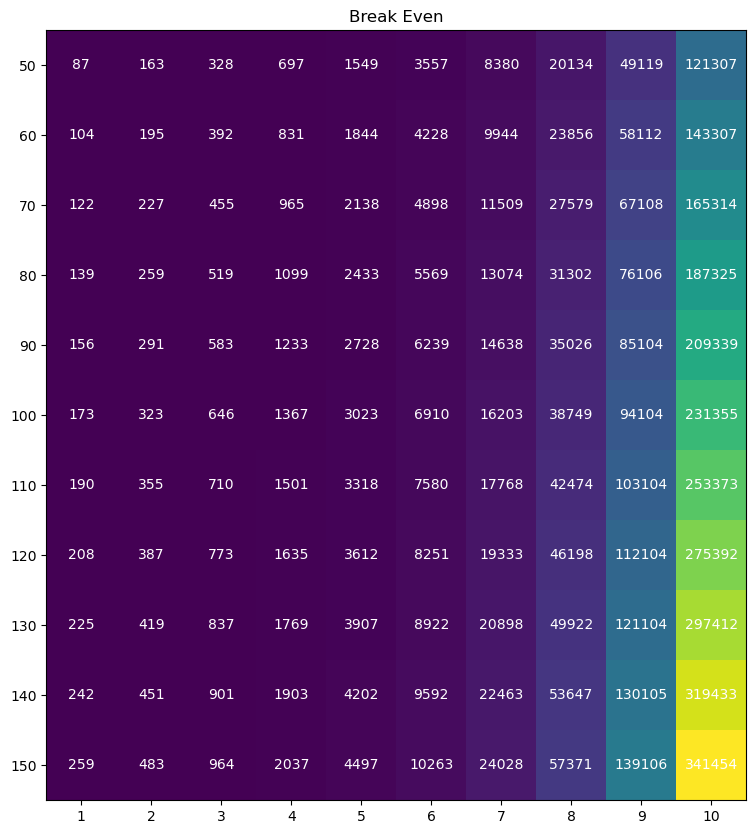
\includegraphics[width=\linewidth]{assets/heatmap-breakeven.png}
  \caption{Heatmap of Break Even.}
  \label{fig:heatmap-breakeven}
\end{figure}

In order to depict the relationship between different values of $W_0$ and $W_1$, a heatmap Figure \ref{fig:heatmap-breakeven} is constructed. As $W_0$ and $W_1$ increase, the number of required event triggers for break even tends to increase. It is suggested to define the values of $W_0$ and $W_1$ based on the download count of an outstanding article. By using this approach, the break even point can be optimized, ensuring a sufficient number of event triggers to achieve equilibrium.
% 根据不同的w0和w1，绘制热力图 1，随着w0和w1的增大，收支平衡的需要事件触发的次数就会越多。此时可以可按照一个优秀论文的下载量来定义w0，和w1值。 


\begin{table*}[ht!]
  \begin{center}
    \caption{Finance for DAO.}
    \label{tab:finance}
    \begin{tabular}{r|l|l|l|l|l|l|l|l|l} % <-- Alignments: 1st column left, 2nd middle and 3rd right, with vertical lines in between
                     & \multicolumn{4}{c|}{\textbf{Authors}} & \textbf{Publisher} & \multicolumn{2}{c|}{\textbf{Reviewers}} & \multicolumn{2}{c}{\textbf{Readers}}                                                                                                    \\
      \hline
      \textbf{index} & \textbf{Corresponding}                & \textbf{Author1}   & \textbf{Author2}                        & \textbf{Author3}                     & \textbf{Publisher} & \textbf{Reviewer1} & \textbf{Reviewer2} & \textbf{Download} & \textbf{Cite} \\
      \hline
      0              & 0.122997                              & 0.184696           & 0.061298                                & 0.030449                             & 0.200321           & 0.177885           & 0.222356           & 0                 & 0             \\
      1              & 0.124113                              & 0.186367           & 0.061860                                & 0.029945                             & 0.197006           & 0.174941           & 0.218676           & 0.007092          & 0             \\
      2              & 0.125194                              & 0.187984           & 0.062403                                & 0.029457                             & 0.193798           & 0.172093           & 0.215116           & 0.006977          & 0             \\
      3              & 0.125000                              & 0.187688           & 0.062312                                & 0.028529                             & 0.187688           & 0.166667           & 0.208333           & 0.006757          & 0.013514      \\
      4              & 0.126016                              & 0.189209           & 0.062823                                & 0.028086                             & 0.184775           & 0.164080           & 0.205100           & 0.006652          & 0.013304      \\
      5              & 0.127001                              & 0.190684           & 0.063319                                & 0.027656                             & 0.181951           & 0.161572           & 0.201965           & 0.006550          & 0.013100      \\
      6              & 0.127957                              & 0.192115           & 0.063799                                & 0.027240                             & 0.179211           & 0.159140           & 0.198925           & 0.006452          & 0.012903      \\
      7              & 0.128884                              & 0.193503           & 0.064266                                & 0.026836                             & 0.176554           & 0.156780           & 0.195975           & 0.006356          & 0.012712      \\
      8              & 0.129784                              & 0.194850           & 0.064718                                & 0.026444                             & 0.173974           & 0.154489           & 0.193111           & 0.006263          & 0.012526      \\
      9              & 0.130658                              & 0.196159           & 0.065158                                & 0.026063                             & 0.171468           & 0.152263           & 0.190329           & 0.006173          & 0.012346      \\
      10             & 0.131508                              & 0.197431           & 0.065585                                & 0.025693                             & 0.169033           & 0.150101           & 0.187627           & 0.006085          & 0.012170      \\
      11             & 0.132333                              & 0.198667           & 0.066000                                & 0.025333                             & 0.166667           & 0.148000           & 0.185000           & 0.006000          & 0.012000      \\
      12             & 0.133136                              & 0.199869           & 0.066404                                & 0.024984                             & 0.164366           & 0.145957           & 0.182446           & 0.005917          & 0.011834      \\
      13             & 0.133917                              & 0.201038           & 0.066796                                & 0.024643                             & 0.162127           & 0.143969           & 0.179961           & 0.005837          & 0.011673      \\
      14             & 0.134677                              & 0.202175           & 0.067179                                & 0.024312                             & 0.159949           & 0.142035           & 0.177543           & 0.005758          & 0.011516      \\
      15             & 0.134268                              & 0.201558           & 0.066978                                & 0.023676                             & 0.155763           & 0.138318           & 0.172897           & 0.005607          & 0.011215      \\
      16             & 0.134994                              & 0.202645           & 0.067343                                & 0.023370                             & 0.153752           & 0.136531           & 0.170664           & 0.005535          & 0.011070      \\
      17             & 0.135701                              & 0.203704           & 0.067699                                & 0.023072                             & 0.151791           & 0.134791           & 0.168488           & 0.005464          & 0.010929      \\
      18             & 0.136391                              & 0.204736           & 0.068046                                & 0.022782                             & 0.149880           & 0.133094           & 0.166367           & 0.005396          & 0.010791      \\
      19             & 0.137063                              & 0.205743           & 0.068384                                & 0.022499                             & 0.148017           & 0.131439           & 0.164298           & 0.005329          & 0.010657      \\
      20             & 0.137719                              & 0.206725           & 0.068713                                & 0.022222                             & 0.146199           & 0.129825           & 0.162281           & 0.005263          & 0.010526      \\
      Total          & 2.749313                              & 4.127544           & 1.371082                                & 0.543292                             & 3.574286           & 3.173966           & 3.967458           & 0.121463          & 0.214788      \\
    \end{tabular}
  \end{center}
\end{table*}


In addition to the theoretical framework, there need conducted simulations to evaluate the effectiveness of the proposed DAO system \cite{macal2009agent}. Table \ref{tab:finance} presents results from 20 simulated downloads, illustrating the distribution of finance among holders. This simulation provides a comprehensive overview of how finance is allocated to holders based on their token holdings \cite{liu2023incremental}. And did data visualization processing \cite{few2004show}.
Within the DAO framework, authors, as the owners of the articles, experience an increase in their tokens and ownership ratio when their articles are downloaded or cited, leading to higher profits. Reviewers, as participants in the article review process, initially receive tokens that do not increase over time. Although their ownership ratio gradually decreases, their profits continue to increase. The accuracy of their ratings directly benefits themselves. Readers, during the process of downloading and citing, also receive tokens, albeit in smaller quantities and with lower ownership ratios. However, as the articles are downloaded or cited, their overall profits increase. Additionally, the profit margin gradually decreases, meaning that readers who download and cite the articles in the early stages will benefit from higher profits, thus incentivizing the early identification of outstanding articles.
%在论文中，我们不仅提出了理论框架，还进行了模拟实验来评估提出的DAO系统的有效性。表格1展示了20次模拟下载的结果，说明了finance在持有者之间的分配情况。这个模拟提供了一个全面的概述，说明了根据令牌持有情况如何分配finance。
% 在这个dao框架之下，author作为文章的拥有者，在文章被下载或被引用时，其token会增加，并且占有率也在增加，同时收益就会越来越高。reviewer作为文章的参与者，他们初期会收到相应的token，但是不再增加，虽然占比逐渐降低，但是收益总是是增加的，评分越准，对自己越有利。reader在download以及cite过程中，都会收到相应的token，虽然量少，并且占有率也不高，但是随着文章被下载或被引用，总收益就也会越来越高。并且在这个过程中，收益率是逐渐下降的，也就是在论文早期下载和引用的reader，会活动比较高的收益，这鼓励了早期识别优秀的论文。


\subsection{Proportion of Trend}


\begin{figure}[h]
  \centering
  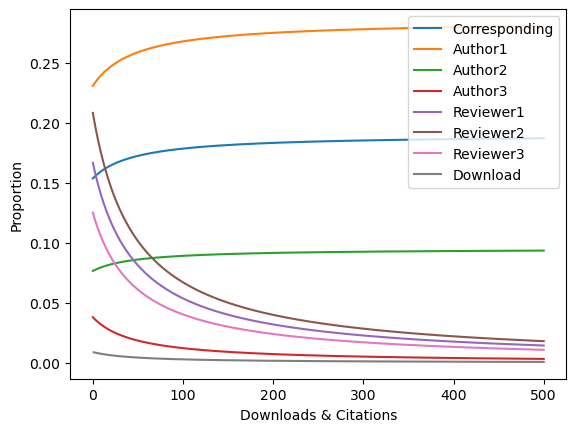
\includegraphics[width=3.2in]{assets/proportion-all.png}
  \caption{Proportion of All.}
  \label{fig:proportion-all}
\end{figure}

Integrating DAO technology into the realm of academic journals holds immense potential for benefiting authors, reviewers, and readers alike. Look at Figure \ref{fig:proportion-all}.
Authors, being the rightful owners of their published works, would reap the most substantial rewards from such a system. By leveraging the decentralized nature of DAOs, authors can secure a greater share of the financial gains associated with their articles. As time progresses, their earnings could potentially increase, providing a long-term incentive for continued contributions.
Reviewers, as the gatekeepers and custodians of scholarly integrity, would also stand to gain from the implementation of DAOs in journals. Initially, they would hold a higher proportion of benefits, reflecting their crucial role in the early stages of article evaluation. However, as time progresses and articles are published, their share of benefits may gradually diminish, ensuring a fair distribution of rewards among all stakeholders.
Readers, as active participants in the scholarly discourse, would also have the opportunity to benefit from DAO-operated journals. While their gains may be comparatively lower than authors and reviewers, early engagement with the DAO ecosystem could yield higher returns. By accessing articles and participating in the DAO's governance processes, readers can contribute to the growth and success of the journal, potentially increasing their benefits over time.
The implementation of DAO mechanisms, such as token-based incentives, transparent governance structures, and decentralized decision-making processes, would enable a fair and equitable model for academic journals. This model fosters a sense of ownership, rewards active participation, and ensures the sustainability and long-term viability of the journal ecosystem.
%将 DAO 技术整合到学术期刊领域具有巨大的潜力，可以使作者、审稿人和读者受益
%作者作为其已发表作品的合法所有者，将从这样的系统中获得最丰厚的回报。通过利用 DAO 的去中心化性质，作者可以获得与其文章相关的更大份额的经济收益。随着时间的推移，他们的收入可能会增加，从而为持续贡献提供长期激励。
%审稿人作为学术诚信的看门人和守护者，也将从期刊中 DAO 的实施中获益。最初，他们将获得较高比例的收益，这反映了他们在文章评估的早期阶段的关键作用。然而，随着文章的发布，他们的利益份额可能会逐渐减少，从而确保所有利益相关者之间公平分配奖励。
%读者作为学术讨论的积极参与者，也将有机会从 DAO 运营的期刊中受益。虽然他们的收益可能相对低于作者和审稿人，但早期参与 DAO 生态系统可能会产生更高的回报。通过访问文章并参与 DAO 的治理流程，读者可以为期刊的发展和成功做出贡献，并有可能随着时间的推移增加其收益。
%DAO 机制的实施，例如基于代币的激励、透明的治理结构和去中心化的决策流程，将为学术期刊提供公平公正的模式。这种模式培养主人翁意识，奖励积极参与，并确保期刊生态系统的可持续性和长期生存能力。



\subsection{Break Even of User Download}

Indeed, allowing users to offset their expenses or even earn profits through downloading articles can effectively stimulate user participation. While individual reader earnings may be modest, readers constitute the largest group within the DAO framework, making them a critical factor for the system's autonomy.
By providing readers with the opportunity to offset their expenses or earn profits, the DAO framework can incentivize their active engagement. Despite individual earnings being relatively small, the cumulative impact of a large number of readers participating in the ecosystem contributes significantly to the overall success and sustainability of the DAO \cite{leimeister2010collective}. As a result, readers play a crucial role in driving the self-governing nature of the DAO framework.
% 用户作为读者下载文章，虽然需要付费，但是如果后面会收支相抵，甚至赚钱，会有效的刺激用户参与。虽然单个reader收益很少，但是在整个DAO框架中，数量最大，是DAO可以可以自治的核心因素。

\begin{figure}[h]
  \centering
  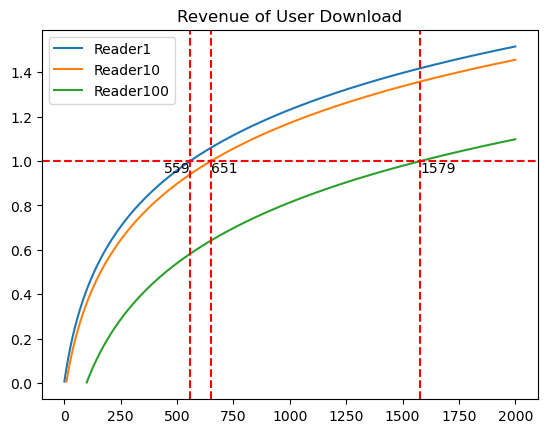
\includegraphics[width=3.2in]{assets/revenue-user-download.png}
  \caption{Revenue of User Download.}
  \label{fig:revenue-user-download}
\end{figure}

The total revenue for downloading users is depicted in Figure \ref{fig:revenue-user-download}. As readers who own the downloaded articles, their total revenue increases with a growing number of users downloading the articles. However, as more readers download the article and become owners, the individual token proportion naturally decreases as Equation \ref{eq:evenotherreader}. Consequently, the per-download revenue gradually declines.
To simulate the distribution ratios following scenario, mainly look at the key break-even points\cite{norreklit2000balance}: the first reader who downloads the article breaks even when the article is downloaded 559 times; the tenth reader breaks even when the article reaches 651 downloads; and the one hundredth reader breaks even at a staggering 1579 downloads. This incentive mechanism aims to encourage readers to discover exceptional articles earlier rather than following the crowd since owning the article no longer yields significant returns.
This approach incentivizes readers to identify outstanding articles sooner, as the potential for substantial earnings diminishes once an article has already demonstrated its quality.
% 下载用户的总收益如图 \ref{fig:revenue-user-download} 所示，随着更多用户下载article，作为读者的article拥有者，总收益会越来越多，但是因为更多其他读者下载article也获取了token，成为了article的拥有者，自己token的占比势必会减少，所以单次收益逐渐降低。设定分配比例进行模拟，第一个下载论文的读者，在文章被下载559次时，总收入与下载时的支出持平；第十个下载论文的读者，收支相抵时候需要文章被下载651次；第一百个下载论文的读者，收支相抵更是要到1579次。此种激励方式在于，如果文章已经证明很优秀了，再拥有已经不能得到多少收益了，鼓励读者更早发现优秀的文章，而不是跟风。


\subsection{Real Article simulation}


\begin{table*}[t!]
  \begin{center}
    \caption{Finance of Real Article for DAO.}
    \label{tab:realpaper}
    \begin{tabular}{r|l|l|l|l|l|l|l|l|l} % <-- Alignments: 1st column left, 2nd middle and 3rd right, with vertical lines in between
                     & \multicolumn{4}{c|}{\textbf{Authors}} & \textbf{Publisher} & \multicolumn{2}{c|}{\textbf{Reviewers}} & \multicolumn{2}{c}{\textbf{Readers}}                                                                                                    \\
      \hline
      \textbf{index} & \textbf{Corresponding}                & \textbf{Author1}   & \textbf{Author2}                        & \textbf{Author3}                     & \textbf{Publisher} & \textbf{Reviewer1} & \textbf{Reviewer2} & \textbf{Download} & \textbf{Cite} \\
      \hline
      0              & 0.122997                              & 0.184696           & 0.061298                                & 0.030449                             & 0.200321           & 0.177885           & 0.222356           & 0                 & 0             \\
      1              & 0.124113                              & 0.186367           & 0.061860                                & 0.029945                             & 0.197006           & 0.174941           & 0.218676           & 0.007092          & 0             \\
      2              & 0.125194                              & 0.187984           & 0.062403                                & 0.029457                             & 0.193798           & 0.172093           & 0.215116           & 0.006977          & 0             \\
      3              & 0.126240                              & 0.189550           & 0.062929                                & 0.028986                             & 0.190694           & 0.169336           & 0.211670           & 0.006865          & 0             \\
      4              & 0.127252                              & 0.191066           & 0.063438                                & 0.028529                             & 0.187688           & 0.166667           & 0.208333           & 0.006757          & 0             \\
      ...            & ...                                   & ...                & ...                                     & ...                                  & ...                & ...                & ...                & ...               & ...           \\

      998            & 0.184995                              & 0.277503           & 0.092486                                & 0.001690                             & 0.011121           & 0.009876           & 0.012345           & 0.000400          & 0.000801      \\
      999            & 0.185000                              & 0.277511           & 0.092489                                & 0.001689                             & 0.011111           & 0.009867           & 0.012333           & 0.000400          & 0.000800      \\
      1000           & 0.185005                              & 0.277519           & 0.092491                                & 0.001687                             & 0.011101           & 0.009857           & 0.012322           & 0.000400          & 0.000799      \\
      1001           & 0.185010                              & 0.277526           & 0.092494                                & 0.001686                             & 0.011090           & 0.009848           & 0.012310           & 0.000399          & 0.000799      \\
      1002           & 0.185015                              & 0.277534           & 0.092497                                & 0.001684                             & 0.011080           & 0.009839           & 0.012299           & 0.000399          & 0.000798      \\

      ...            & ...                                   & ...                & ...                                     & ...                                  & ...                & ...                & ...                & ...               & ...           \\

      2151           & 0.186032                              & 0.279053           & 0.093011                                & 0.000803                             & 0.005285           & 0.004693           & 0.005867           & 0.000190          & 0.000381      \\
      2152           & 0.186034                              & 0.279056           & 0.093012                                & 0.000803                             & 0.005283           & 0.004691           & 0.005864           & 0.000190          & 0.000380      \\
      2153           & 0.186036                              & 0.279059           & 0.093013                                & 0.000803                             & 0.005281           & 0.004689           & 0.005861           & 0.000190          & 0.000380      \\
      2154           & 0.186038                              & 0.279062           & 0.093014                                & 0.000802                             & 0.005278           & 0.004687           & 0.005859           & 0.000190          & 0.000380      \\
      Total          & 392.406327                            & 588.652390         & 196.160264                              & 6.520750                             & 42.899672          & 38.094909          & 47.618636          & 1.537177          & 1.768627      \\
    \end{tabular}
  \end{center}
\end{table*}

Furthermore, we applied our DAO framework to a real-world case by analyzing a published paper with 2154 downloads and 42 citations. As shown in Table \ref{tab:realpaper}. By simulating the income distribution within the current DAO structure \cite{efron1994introduction}, we observed that download users not only offset their initial payment but also gained additional earnings. The incentivized system encourages users to respect copyright and, more importantly, has achieved a level of autonomy.The provided tables and case study demonstrate the practical application and positive outcomes of our proposed DAO framework. By aligning incentives with user behaviors, the system not only offsets costs for downloaders but also significantly incentivizes engagement. This not only respects copyright but also establishes a self-sustainable and autonomous ecosystem, providing valuable insights for the future development of decentralized academic publishing.

%此外，我们将DAO框架应用于一个真实案例，分析了一篇被下载2154次、引用42次的论文。通过模拟当前DAO结构下的收入分配情况，我们观察到下载用户不仅抵消了初始支付，还获得了额外的收益。这个激励系统鼓励用户尊重版权，更重要的是实现了一定程度的自治。提供的表格和案例研究展示了我们提出的DAO框架的实际应用和积极成果。通过将激励与用户行为保持一致，该系统不仅为下载者抵消了成本，还极大地激励了用户参与。这不仅尊重版权，还建立了一个自我可持续和自治的生态系统，为分散的学术出版的未来发展提供了有价值的见解。



After voluntarily making a payment, users' ability to participate contributes to a robust incentive mechanism, fostering a sense of autonomy within the entire framework. Through this design, users become direct contributors to financial activities, injecting new value into the framework and creating potential opportunities for self-reward. This decentralized autonomous model empowers users to engage directly in decision-making and contributions, shaping a more open, fair, and virtuous ecosystem. Overall, this autonomous framework cultivates a more positive and sustainable participation experience for users and the entire community.
Through the detailed simulations and analyses, the incentive mechanisms within the DAO framework emerge as crucial drivers in shaping the dynamics of authorship and user participation. As downloads and citations increase, the token-driven rewards become a powerful motivator for authors, leading to an accumulation of influence and financial gains. This incentive structure not only acknowledges and rewards the contributions of authors but also establishes a direct correlation between their efforts and the benefits they accrue.
Furthermore, users who engage with the system by downloading papers witness a direct impact on their influence and, subsequently, on their earnings. This creates a dual incentive structure, where authors and users are mutually motivated to contribute to and participate in the DAO environment. The concept of decentralized autonomy becomes evident as the system operates independently, fostering a self-sustaining loop of contributions, rewards, and governance.
In this context, the DAO framework provides a powerful tool for aligning interests and promoting a fair distribution of rewards based on tangible contributions. The transparency and automation inherent in DAO contribute to a governance model that minimizes external intervention, allowing the ecosystem to evolve organically through the collective actions of its participants. This synergy of incentives and autonomy within DAO not only enhances the overall efficiency of the academic publishing model but also creates a robust and self-regulating environment for authors and users alike \cite{ostrom1990governing}.
%用户自主付费后，其参与框架的能力构成了一种积极的激励机制，为整个系统的自治性提供了有力支持。通过这一设计，用户成为财务活动的直接贡献者，其行为不仅为框架注入了新的价值，同时也为自身创造了潜在的奖励机会。这种去中心化的自治模式使得用户能够更加直接地参与决策和贡献，从而塑造了一个更加开放、公正、而且具有良性循环的生态系统。整体而言，这种自治的框架为用户和整个社区创造了更为积极和可持续的参与体验。
%通过详尽的模拟和分析，DAO框架内的激励机制成为塑造作者和用户参与动态的关键推动因素。随着下载和引用的增加，基于代币的奖励变得越来越成为作者的强大动力，导致权重和财务收益的积累。这种激励结构不仅承认并奖励了作者的贡献，还在作者的努力和他们获得的收益之间建立了直接的关系。
%此外，通过下载论文积极参与系统的用户在他们的影响力和随之而来的收入上见证了直接的影响。这创建了一个双重的激励结构，使作者和用户相互激励，以在DAO环境中做出贡献和参与。去中心化自治的概念在系统自主运作中变得明显，形成了一个贡献、奖励和治理的自我维持循环。
%在这种情况下，DAO框架为协调利益和促进基于实际贡献的公平奖励分配提供了强大的工具。DAO内在的透明度和自动化有助于最小化外部干预的治理模型，通过参与者的集体行动，使生态系统有机地演变。DAO内的激励和自治的协同作用不仅提升了学术出版模型的整体效率，而且为作者和用户创造了一个强大而自我调节的环境。



% Once the paper is on the blockchain, it unequivocally belongs to the author, author is the real owner,that creating endless possibilities, especially in terms of financial activities. This means that the author not only owns their work but can also leverage blockchain technology to create various financial opportunities. Authors can receive rewards through financial activities, which may include paid downloads, knowledge exchanges, collaborative projects, and more. This decentralized framework provides authors with greater creative freedom and potential economic returns, enabling them to be more independent and influential in the academic domain. Overall, putting a paper on the blockchain opens up a new and forward-thinking path for authors.
% %论文一旦上链，将完全归属于作者，作者就是真正的拥有者，为作者创造了无限的可能性，特别是在财务活动方面。这意味着作者不仅拥有其作品的所有权，而且可以利用区块链技术创造各种财务机会。作者可以通过财务活动获得回报，这可能包括付费下载、知识交流、合作项目等。这种去中心化的框架为作者提供了更大的创作自由和潜在的经济回报，使其在学术领域更加独立和有影响力。整体而言，论文上链为作者开辟了一个全新的、具有前瞻性的创作道路。



\section{Conclusion \label{sec:conclusion}}
This paper delves into the framework of DAOs and provides a comprehensive analysis of their potential applications in academic publishing. By utilizing recursive inscriptions, it overcomes blockchain limitations, making inscriptions a key evaluative parameter for both articles and reviewers. By integrating academic articles onto the blockchain, we achieve transparency in ownership, enabling authors to fully control their work while generating significant financial opportunities. The autonomous nature of DAOs allows users to directly participate in decision-making and contribute to the ecosystem, creating an open, fair, and autonomous system. Within this framework, users are rewarded with tokens during minting events, based on detailed inscriptions. These tokens not only grant users increased decision-making power but also provide sustainable income streams. Lastly, ordinary readers are granted the right to earn tokens, fostering the spread of paid knowledge and encouraging greater participation in the knowledge economy.

%本文深入探讨了去中心化自治组织（DAO）的框架，并就其在学术出版领域的潜在应用进行了详尽分析。首先使用递归铭文，突破了区块链的限制，并且让铭文成为了文章和审稿人的重要评判参数。通过将论文上链，我们实现了论文所有权的透明化，使作者能够完全拥有其作品，同时也为其创造了丰富的财务机会。DAO的自治性质使得用户能够直接参与决策和贡献，构建了一个开放、公正、具有良性循环的生态系统。在这一框架下，用户通过细化的铭文在铸币事件得到了token作为回报，这会给用户更高的决策权重，还给了用户创造了可持续的收入。最后，给了普通读者获得token的权利，这会促进知识付费的传播。



Once a paper is uploaded to the blockchain, it opens up limitless possibilities for the future, and the application of DAOs will continue to expand. The potential extensions of NFTs and recursive inscriptions go far beyond their current uses, with many more innovative applications emerging within the DAO ecosystem. These new applications will further drive the development of DeSci, fostering greater collaboration, transparency, and innovation in the academic and scientific communities. As DAO frameworks evolve, they will play a pivotal role in transforming how knowledge is shared, validated, and monetized, shaping the future of decentralized research and publication.
% 文章一旦上链，未来就有了无限可能，DAO的应用将会越来越广泛。在NFT以及递归铭文上的扩展远不止如此，还有更多的新应用在DAO生态系统中出现，这些新的应用将会促进DeSci的发展。


\bibliography{refs}
\bibliographystyle{IEEEtran}


\newpage



\begin{IEEEbiography}[{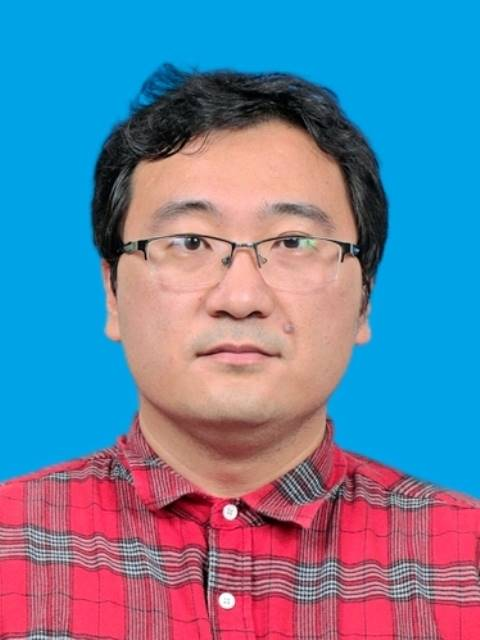
\includegraphics[width=1in,height=1.25in,clip,keepaspectratio]{assets/thales.jpg}}]{Tai Jiang}
  received the master’s degree in Master of Business Administration from the University of Chinese Academy of Sciences, Beijing, in 2022, where he is currently pursuing the Ph.D. degree with the Institute of System Engineering, Macau University of Science and Technology, Macao, China.

  he is with the Department of Engineering Science, Faculty of Innovation Engineering, Macau University of Science and Technology, Macao, 999078, China. His research interests include parallel intelligence, blockchain, DAOs, NFTs, Meta, and Decentralized Science.
\end{IEEEbiography}

\vspace{-33pt}

\begin{IEEEbiography}[{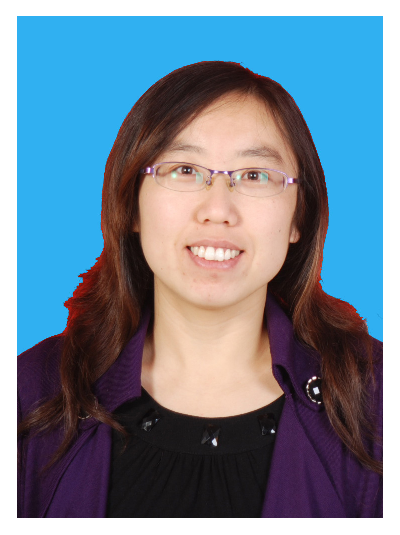
\includegraphics[width=1in,height=1.25in,clip,keepaspectratio]{assets/Rui.eps}}]{Rui Qin}
  (Member, IEEE) received the Ph.D. degree in computer application technology from the University of Chinese Academy of Sciences, Beijing, China, in 2016.

  She is currently an Associate Professor with State Key Laboratory of Multimodal Artificial Intelligence Systems, Institute of Automation, Chinese Academy of Sciences, Beijing. Her research interests include blockchain, DAO, and parallel management.
\end{IEEEbiography}

\vspace{-33pt}

\begin{IEEEbiography}[{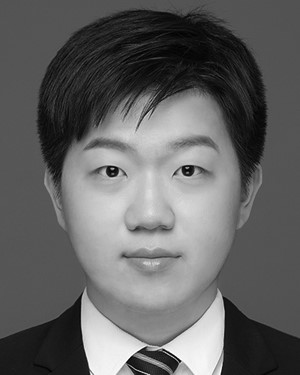
\includegraphics[width=1in,height=1.25in,clip,keepaspectratio]{assets/yhliu.jpg}}]{Yuhang Liu}
  received the B.S. degree from the Department of Precision Instruments, Tsinghua University, Beijing, China, in 2021. He is currently working toward the Ph.D. degree with the Institute of Automation, Chinese Academy of Sciences, Beijing. His research interests include parallel radars, 3D object detection, and point cloud data generation.
\end{IEEEbiography}

\vspace{-33pt}

\begin{IEEEbiography}[{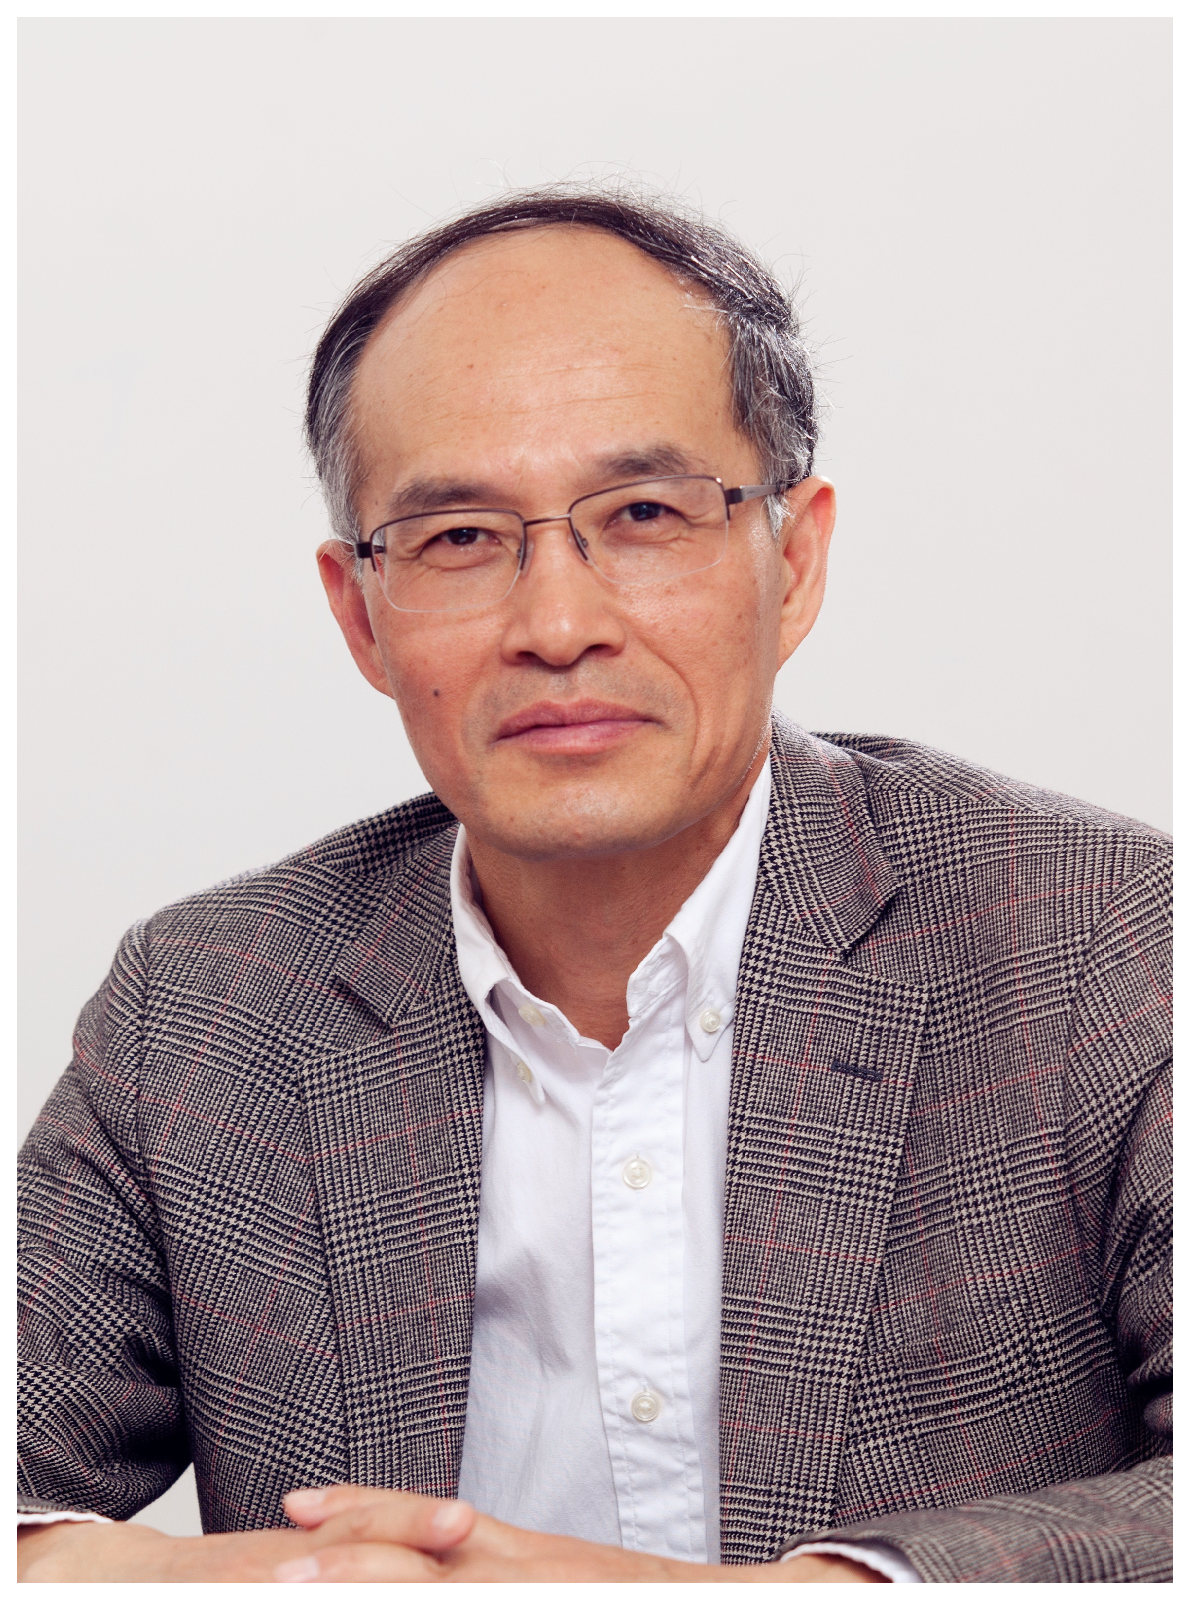
\includegraphics[width=1in,height=1.25in,clip,keepaspectratio]{assets/FW.eps}}]{Fei-Yue Wang} (S’87–M’89–SM’94–F’03)
  received his Ph.D. degree in computer and systems engineering from the Rensselaer Polytechnic Institute, Troy, NY, USA, in 1990. He joined The University of Arizona in 1990 and became a Professor and the Director of the Robotics and Automation Laboratory and the Program in Advanced Research for Complex Systems. In 1999, he founded the Intelligent Control and Systems Engineering Center at the Institute of Automation, Chinese Academy of Sciences (CAS), Beijing, China, under the support of the Outstanding Chinese Talents Program from the State Planning Council, and in 2002, was appointed as the Director of the Key Laboratory of Complex Systems and Intelligence Science, CAS, and Vice President of Institute of Automation, CAS in 2006. He found CAS Center for Social Computing and Parallel Management in 2008, and became the State Specially Appointed Expert and the Founding Director of the State Key Laboratory for Management and Control of Complex Systems in 2011. He is a distinguished professor at the Macau University of Science and Technology.

  His current research focuses on methods and applications for parallel intelligence, social computing, and knowledge automation. He is a Fellow of International Council on Systems Engineering (INCOSE), International Federation of Automatic Control (IFAC), American Society of Mechanical Engineers (ASME), and American Association for the Advancement of Science (AAAS). In 2007, he received the National Prize in Natural Sciences of China, numerous best papers awards from IEEE Transactions, and became an Outstanding Scientist of Association for Computing Machinery(ACM) for his work in intelligent control and social computing. He received the IEEE Intelligent Transportation Systems (ITS) Outstanding Application and Research Awards in 2009, 2011, and 2015, respectively, the IEEE Systems, Man, and Cybernetics Society (SMC) Norbert Wiener Award in 2014, and became the IFAC Pavel J. Nowacki Distinguished Lecturer in 2021.

  Since 1997, he has been serving as the General or Program Chair of over 30 IEEE, Institute for Operations Research and the Management Sciences (INFORMS), IFAC, ACM, and ASME conferences. He was the President of the IEEE ITS Society from 2005 to 2007, the IEEE Council of Radio Frequency Identification (RFID) from 2019 to 2021, the Chinese Association for Science and Technology, USA, in 2005, the American Zhu Kezhen Education Foundation from 2007 to 2008, the Vice President of the ACM China Council from 2010 to 2011, the Vice President and the Secretary General of the Chinese Association of Automation (CAA) from 2008 to 2018, the Vice President of IEEE SMC from 2019 to 2021. He was the Founding Editor-in-Chief (EiC) of the International Journal of Intelligent Control and Systems from 1995 to 2000, IEEE ITS Magazine from 2006 to 2007, JOURNAL OF AUTOMATICA SINICA (IEEE/CAA) from 2014-2017, China's Journal of Command and Control from 2015-2021, and China's Journal of Intelligent Science and Technology from 2019 to 2021. He was the EiC of the IEEE Intelligent Systems from 2009 to 2012, IEEE TRANSACTIONS on ITS from 2009 to 2016, IEEE TRANSACTIONS ON COMPUTATIONAL SOCIAL SYSTEMS from 2017 to 2020. Currently, he is the President of CAA's Supervision Council, and the EiC of IEEE Trans. on Intelligent Vehicles.
\end{IEEEbiography}



\vfill

\end{document}


